\documentclass{report}[11pt]
\usepackage{graphicx}
\usepackage[hungarian]{babel}
\usepackage{float}
\usepackage{t1enc}
\usepackage[export]{adjustbox}
\usepackage{hyperref}
\usepackage{listings}
\usepackage{xcolor}
\usepackage{float}

\begin{document}
% Define C# syntax highlighting
\lstdefinelanguage{CSharp}{
    morekeywords={abstract, event, new, struct, as, explicit, null, switch, base, extern, object, 
        this, break, false, operator, throw, byte, finally, out, true, case, fixed, override, try, 
        catch, float, params, typeof, char, for, private, uint, checked, foreach, protected, ulong, 
        class, goto, public, unchecked, const, if, readonly, unsafe, continue, implicit, ref, ushort, 
        decimal, in, return, using, default, int, sbyte, virtual, delegate, interface, sealed, volatile, 
        do, internal, short, void, double, is, sizeof, while, dynamic, lock, stackalloc, else, long, 
        static, enum, namespace, string},  
    sensitive=true,
    morecomment=[l]{//},
    morecomment=[s]{/*}{*/},
    morestring=[b]",
    morestring=[b]'
}

\lstset{
    language=CSharp,
    basicstyle=\ttfamily\small,
    keywordstyle=\color{blue},
    stringstyle=\color{red},
    commentstyle=\color{gray}\ttfamily\itshape,
    numbers=left,
    numberstyle=\tiny\color{gray},
    stepnumber=1,
    breaklines=true,
    tabsize=4,
    captionpos=b
}


	\begin{titlepage}
		\begin{center}
			
\includegraphics[width=30mm,keepaspectratio]{figures/mechwart_logo.png}\\
			\vspace{0.3cm}
			\textbf{DSZC Mechwart András Gépipari és Informatikai Technikum}\\
			\textmd{13.C}\\
			\textmd{Szoftverfejlesztő és -tesztelő ágazat}\\[3cm]
			\vspace{0.2cm}
			{\huge \bfseries PremiumCars Használtautó-kereskedelmi hálózat fejlesztői dokumentációja. }\\[0.8cm]
			\vspace{0.5cm}
			\textsc{\Large Vizsgaremek }\\[4cm]
			\renewcommand{\arraystretch}{0.85}
			\begin{tabular}{cc}
                \makebox[5cm]{\emph{Készítette}} & \makebox[5cm]{\emph{Készítette}} \\
                \noalign{\smallskip}
                \makebox[5cm]{Gál Bálint Szelim} & \makebox[5cm]{Kiss Dániel}
            \end{tabular}            
			\vfill
			{\large \today}
		\end{center}
	\end{titlepage} 
    \tableofcontents \newpage
    
    \chapter{Bevezetés}

    A jelen vizsgaremekben bemutatott rendszer egy autókereskedési platform, mely célja, hogy hatékony és felhasználóbarát megoldást kínáljon a használt autók online értékesítésére és kezelésére. A projekt a \textit{PremiumCars} névre hallgat, és lehetőséget biztosít a felhasználók számára autók mentésére, keresésére, valamint a hozzájuk kapcsolódó adatkezelésre, mint például a mentett autók listázása és törlése.
    
    A téma választásának indoklása részben a személyes érdeklődésen alapul, mivel a szoftverfejlesztés, különösen az üzleti alkalmazások fejlesztése iránti vágy mindig is jelen volt. Azonban a projekt iránti érdeklődésem egyik fő motivációja az volt, hogy Magyarországon rendkívül ritka az olyan típusú autókereskedelmi modell, amely online platformot biztosít a használt autók értékesítésére. Ez a gondolat akkor kezdett el formálódni, amikor meglátogattam egy \textit{WeCars} autókereskedőt Japánban. Bár használt autókról volt szó, az ott tapasztalt élmény azt a benyomást keltette bennem, mintha egy vadonatúj autót vásárolnék. Az autókereskedés a minőségi szolgáltatásaival és professzionális hozzáállásával egy olyan vásárlási élményt nyújtott, amely messze túlmutatott a hagyományos használt autópiaci elvárásokon. Ez az élmény és a japán piac hatása inspirálta a projektet.
    
    A projekt tehát elsősorban a japán piacra összpontosít, figyelembe véve a helyi autókereskedelmi trendeket, mint például a \textit{WeCars} és más hasonló cégek működését. Azonban a fejlesztés során figyelembe vettük, hogy a rendszer egy kis átalakítással a magyar piacra is alkalmazható lehet. A japán autópiacra jellemző szolgáltatási szint és vásárlói élmény például inspiráló lehet Magyarország számára is, ahol a használt autók értékesítése gyakran kisebb vállalkozások körében zajlik, és az online platformok még nem elterjedtek.
    
    A szakmai célkitűzés a projektben, hogy egy olyan zökkenőmentes, könnyen kezelhető platformot biztosítson, amely egyszerűsíti az autóvásárlás és -értékesítés folyamatát. A rendszer valós üzleti környezetben alkalmazható megoldásokat céloz, és nemcsak az autókereskedők, hanem a vásárlók számára is értékes lehetőségeket kínál. A téma tehát egy aktuális és gyakorlati probléma megoldására tett kísérlet, amely mind a fejlesztő, mind a felhasználók számára hasznos tapasztalatokat biztosít, és a jövőben akár a magyar autópiacon is sikeres lehet.
    
    \chapter{Csapatmunka}
    \section{Csapatmunka és Kommunikáció}

A projekt fejlesztése során a csapattagok napi szinten együtt dolgoztak, így a személyes kommunikáció volt a legfontosabb eszköz. Emellett online platformokat is használtunk a hatékony munkavégzés és a fejlesztési folyamatok követése érdekében.

\subsubsection{Kommunikációs Eszközök}

\begin{itemize}
    \item \textbf{Személyes együttműködés} – Mivel napi 8 órát együtt töltöttünk a fejlesztés során, a legtöbb probléma megbeszélésére és megoldására azonnal sor kerülhetett. Ez jelentősen gyorsította a fejlesztési folyamatot.
    \item \textbf{Discord} – Online megbeszélésekhez és képernyőmegosztásos hibakereséshez használtuk, amikor nem volt lehetőség személyes találkozásra.
    \item \textbf{Messenger} – Gyors üzenetváltásokhoz és szervezési kérdésekhez használtuk.
    \item \textbf{JIRA} – A feladatok nyomon követésére és a munkafolyamatok strukturálására alkalmaztuk. A fejlesztési feladatokat kisebb egységekre bontottuk, és a státuszukat folyamatosan frissítettük.
\end{itemize}

\subsubsection{Feladatmegosztás}

A csapat két fő fejlesztőből állt, akik egyértelműen meghatározott felelősségi köröket láttak el:

\begin{itemize}
    \item \textbf{Gál Bálint Szelim} – A backend fejlesztéséért, a web API kapcsolatokért és a WPF alkalmazás nagy részéért volt felelős. Az adatbázis-kezelés, az üzleti logika és az API-hívások implementálása az ő feladata volt.
    \item \textbf{Kiss Dániel} – A weboldal frontend fejlesztésének teljes egészéért volt felelős, kivéve az API-hívásokat. Az oldalak struktúrája, a komponensek és a vizuális megjelenés hozzá tartoztak.
\end{itemize}

A személyes együttműködés kulcsszerepet játszott a projekt sikerességében, mivel a folyamatos kommunikáció és az azonnali problémamegoldás lehetővé tette a hatékony fejlesztést.


\chapter{Technológiai választások és fejlesztői eszközök}

\section{Technológiai választások}
A projekt fejlesztése során a következő technológiákat választottuk:

\begin{itemize}
    \item \textbf{C\# .NET 8 Web API} – A backend fejlesztésére használtuk, mivel modern, stabil és jól támogatott keretrendszer, amely lehetővé teszi a gyors fejlesztést.
    \item \textbf{PostgreSQL} – Az adatbáziskezeléshez ezt választottuk, mivel a MySQL használata macOS alatt az Entity Frameworkkel együtt furcsa hibákat eredményezett, amelyek megoldása nem volt ésszerű.
    \item \textbf{React + TypeScript} – A frontend fejlesztéséhez TypeScriptet használtunk, mivel erősebb típusellenőrzést biztosít, ami csökkenti a hibák számát.
    \item \textbf{WPF (Windows Presentation Foundation)} – Az asztali alkalmazás fejlesztésére, mivel lehetővé teszi az MVVM nélküli gyors fejlesztést és jól integrálható a .NET API-val.
\end{itemize}

\section{Fejlesztői eszközök}
A fejlesztés során a következő eszközöket használtuk:

\begin{itemize}
    \item \textbf{JetBrains Rider} – A .NET alkalmazás fejlesztésére választottuk, mivel kiváló támogatást nyújt a C\# és a .NET környezet számára.
    \item \textbf{Visual Studio 2022} – A WPF fejlesztéshez használtuk, mivel teljes körű támogatást nyújt a .NET technológiákhoz és XAML-hez.
    \item \textbf{WebStorm} – A frontend fejlesztéséhez React és TypeScript támogatás miatt.
    \item \textbf{Visual Studio Code} – Könnyűsúlyú szerkesztőként használtuk gyors kódolási feladatokhoz.
    \item \textbf{Navicat Premium} – Az adatbázis kezeléséhez és vizuális tervezéséhez.
    \item \textbf{pgAdmin 4} – Az adatbázis kezeléséhez és az SQL lekérdezések teszteléséhez.
    \item \textbf{Postman} – Az API végpontok teszteléséhez.
    \item \textbf{Git + GitHub} – Verziókezeléshez és csapatmunkához.
\end{itemize}

\section{Külső csomagok és függőségek}
A fejlesztés során a következő külső csomagokat használtuk:

\begin{itemize}
    \item \textbf{AutoMapper (13.0.1)} – Az objektumok közötti automatikus leképezéshez az üzleti logikában.
    \item \textbf{Microsoft.AspNetCore.Authentication.JwtBearer (8.0.11)} – A JWT-alapú hitelesítés kezeléséhez.
    \item \textbf{Microsoft.AspNetCore.Identity.EntityFrameworkCore (8.0.11)} – Az Identity kezeléséhez Entity Framework Core segítségével.
    \item \textbf{Microsoft.EntityFrameworkCore.Proxies (9.0.0)} – Az adatbázis entitások lazy loading funkcióinak támogatásához.
    \item \textbf{Microsoft.EntityFrameworkCore.Tools (9.0.0)} – Az Entity Framework migrációk és adatbáziskezelés támogatásához.
    \item \textbf{Microsoft.EntityFrameworkCore (9.0.0)} – Az adatbázis-kezeléshez és az ORM réteg megvalósításához.
    \item \textbf{Npgsql.EntityFrameworkCore.PostgreSQL (9.0.2)} – A PostgreSQL adatbázis Entity Framework Core támogatásához.
    \item \textbf{Swashbuckle.AspNetCore (6.4.0)} – Az API dokumentáció generálásához Swagger segítségével.
\end{itemize}

\section{Egyéb eszközök és segédprogramok}
A fejlesztés során egyéb eszközöket és saját szkripteket is használtunk a hatékonyabb munkavégzés érdekében:

\begin{itemize}
    \item \textbf{Python szkript tömeges képletöltéshez} – Egy saját Python szkriptet írtunk, amely segített autóhirdetések képeit tömegesen letölteni, hogy az adatbázisban valósághű demóadatokat használhassunk.
    \item \textbf{iTerm2} – A terminálos munkavégzéshez macOS-en.
\end{itemize}

A fent említett technológiák és eszközök együttes használata biztosította a rendszer stabilitását és skálázhatóságát.


    \chapter{Telepítés és konfiguráció}
    \section{Szerver Beállítások}
    
Ez a szakasz bemutatja a Hasznaltauto-kereskedelmi rendszer szerverének beállítási lépéseit.

\subsection{Előfeltételek}
A projekt szerverének futtatásához az alábbi szoftverekre van szükség:
\begin{itemize}
    \item \textbf{.NET 8} - A szerver és a backend fejlesztéséhez.
    \item \textbf{PostgreSQL} - Az adatbázis kezeléséhez.
\end{itemize}

\subsection{Adatbázis Telepítése}
A projekt adatbázisának beállításához importáld a mellékelt adatbázis dump fájlt a PostgreSQL szerveredbe (az új "dealership" adatbázisba):
\begin{itemize}
    \item Töltsd le a dump fájlt a GitHub oldalunkról: \href{https://github.com/suketti/CarDealershipSystem}{A projekt github oldalda}.
    \item Nyisd meg a pgAdmin4-et, és hozd létre a \texttt{dealership} adatbázist.
    \item Importáld a dump fájlt a \texttt{dealership} adatbázisba.
\end{itemize}

\subsubsection{2. Új adatbázis létrehozása}

1. Nyissuk meg \textbf{pgAdmin4}-et, és jelentkezzünk be.
2. A bal oldali menüben kattintsunk a \textbf{Servers} > \textbf{PostgreSQL} elemre.
3. Kattintsunk jobb gombbal a \textbf{Databases} elemre, majd válasszuk az \textbf{Create} > \textbf{Database...} opciót.
4. Az új ablakban adjuk meg az adatbázis nevét, például: \texttt{dealership}.

\begin{figure}[H]
    \centering
    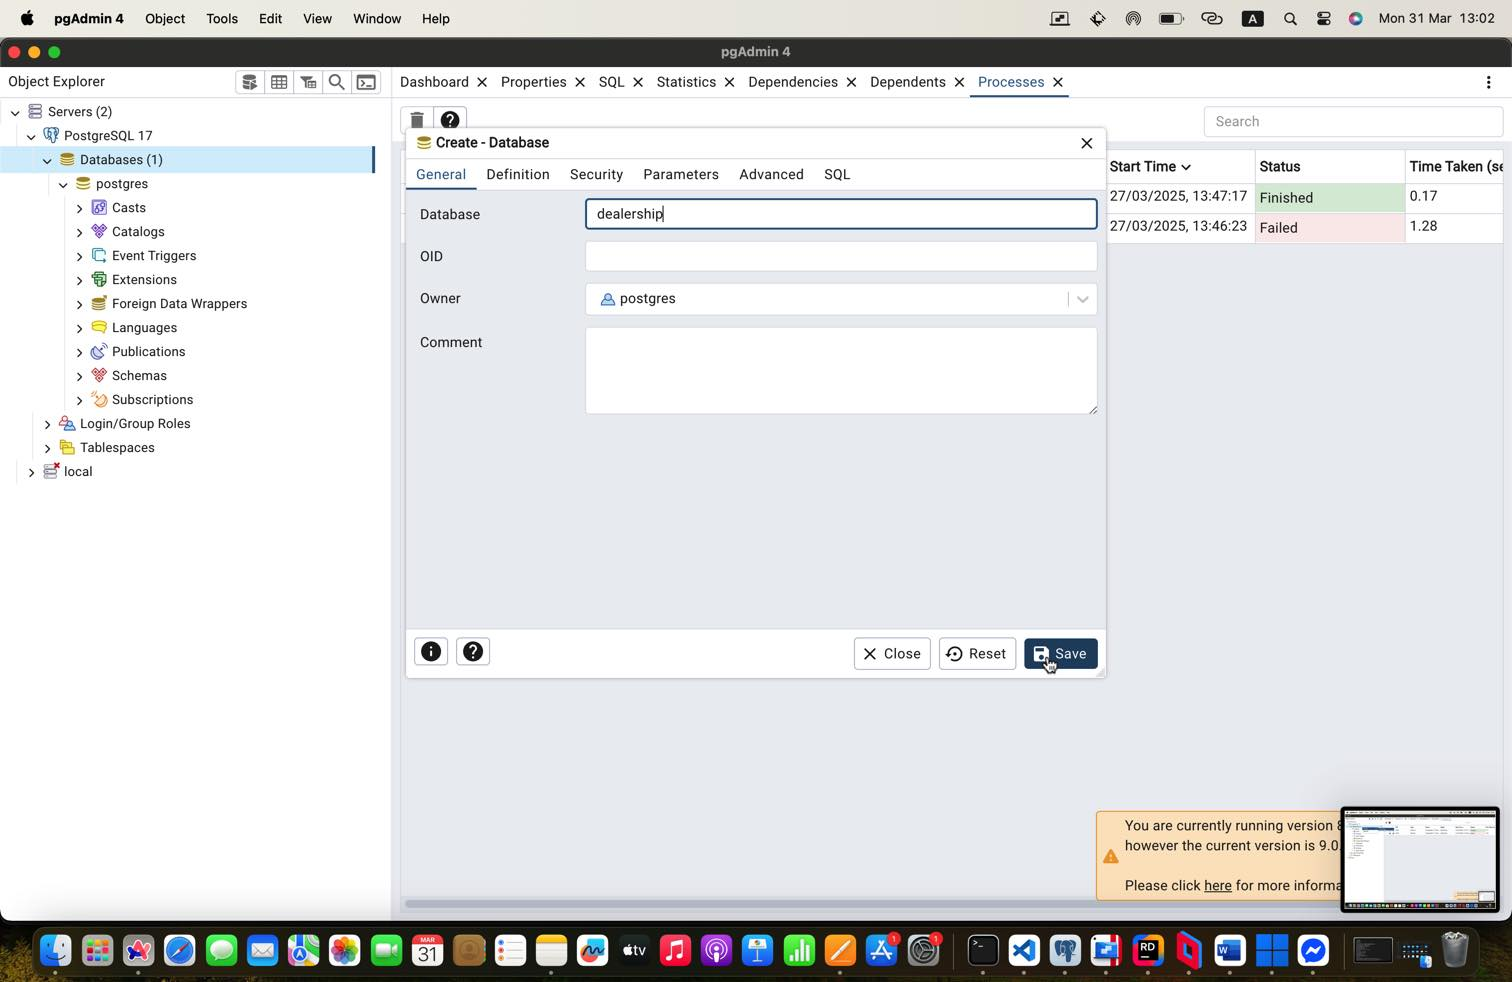
\includegraphics[width=0.8\textwidth]{figures/db_create.png}
    \caption{Új adatbázis létrehozása pgAdmin4-ben}
    \label{fig:create_db}
\end{figure}

5. A \textbf{Save} gombbal hozzuk létre az adatbázist.

\subsubsection{3. Adatbázis dump importálása}

Az adatbázis feltöltéséhez a már meglévő dump fájl segítségével a következő lépéseket kell követni:

1. Nyissuk meg a pgAdmin4-et, és csatlakozzunk a PostgreSQL szerverhez.
2. A bal oldali menüben bontsuk ki a \textbf{Databases} listát, és válasszuk ki az előző lépésben létrehozott \texttt{dealership} adatbázist.
3. Kattintsunk jobb gombbal az adatbázisra, majd válasszuk az \textbf{Restore...} opciót.


4. A megnyíló ablakban:
   \begin{itemize}
       \item A \textbf{Filename} mezőben tallózzuk be az adatbázis dump fájlt (\texttt{dealership\_dump.sql}).
       \item A \textbf{Format} mezőnél válasszuk a \texttt{Custom or tar} opciót, ha a dump fájl bináris formátumú (\texttt{.backup} vagy \texttt{.tar}).
       \item Ha a dump fájl SQL formátumú, válasszuk a \texttt{Plain} formátumot.
   \end{itemize}

   \begin{figure}[H]
    \centering
    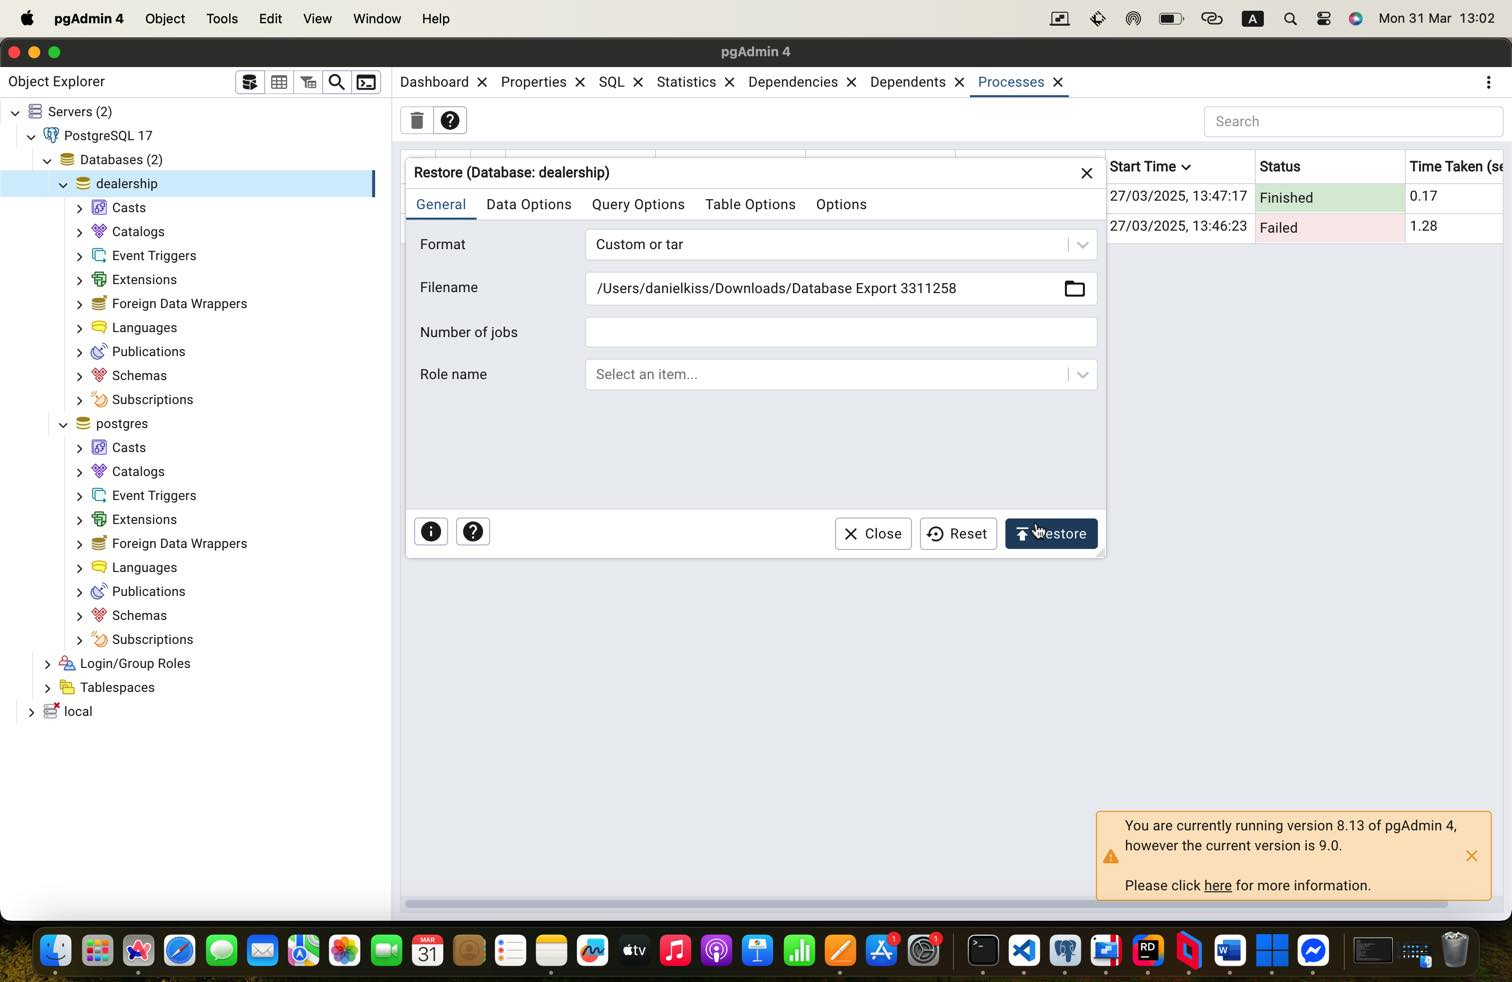
\includegraphics[width=0.8\textwidth]{figures/db_restore.png}
    \caption{Adatbázis visszaállítása (Restore) menü}
    \label{fig:restore_menu}
\end{figure}


5. Kattintsunk a \textbf{Restore} gombra az importálás elindításához.



\begin{figure}[H]
    \centering
    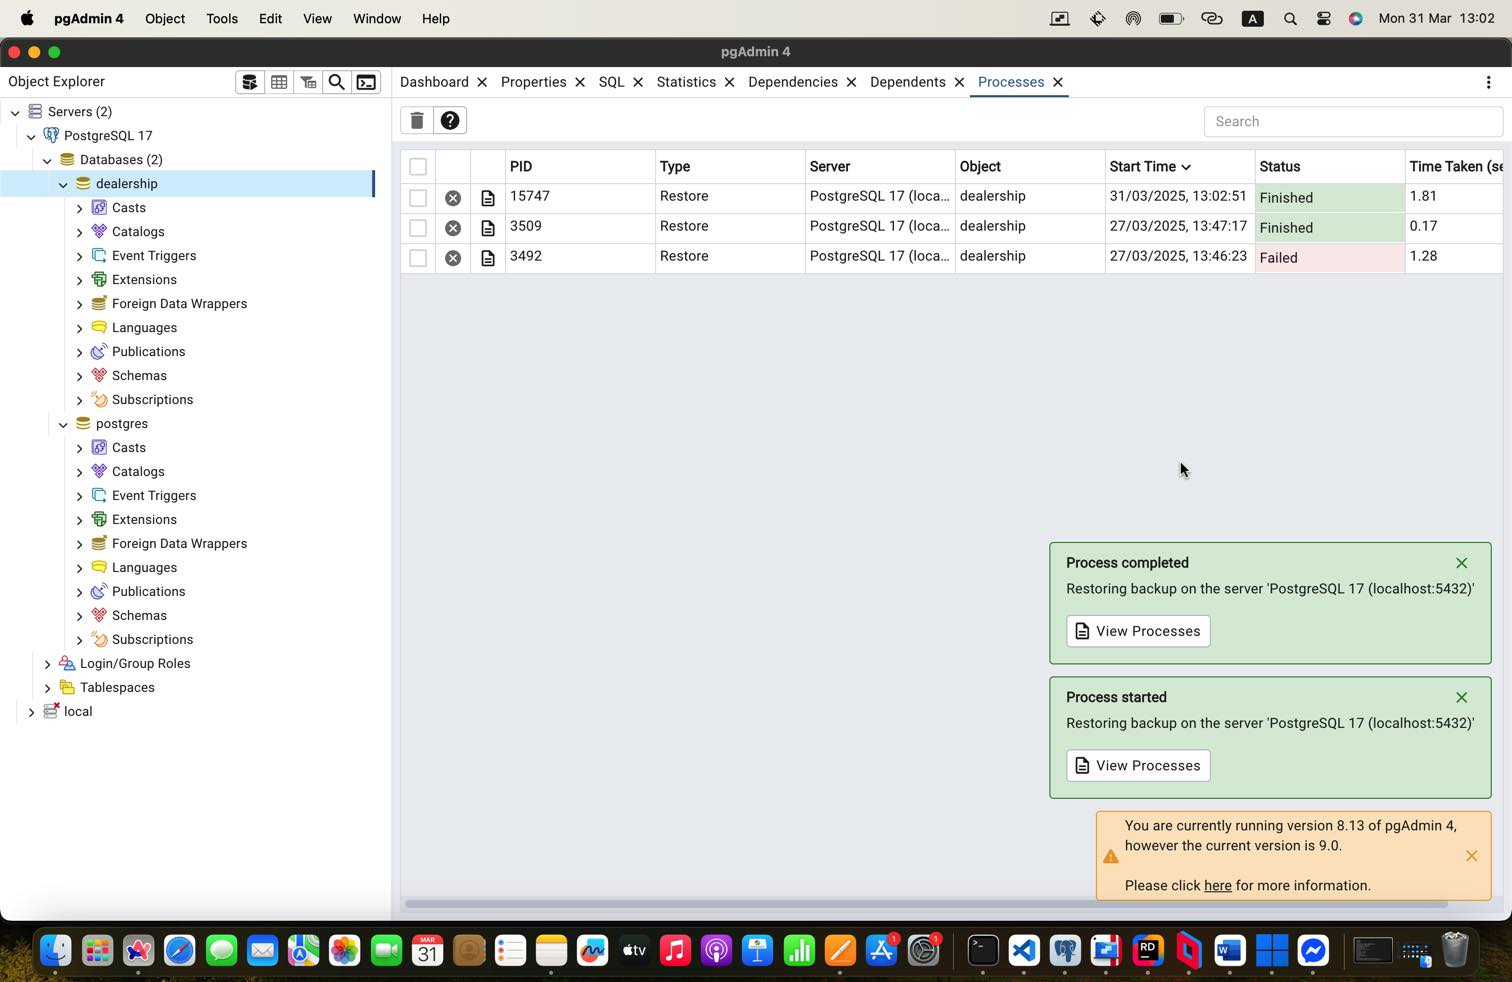
\includegraphics[width=0.8\textwidth]{figures/restore_complete.png}
    \caption{Importálás befejeződött}
    \label{fig:restore_complete}
\end{figure}


\subsection{Szerver Beállítása}
A szerver konfigurálásához módosítanod kell a következő fájlokat:

\subsubsection{appSettings.json}
A \texttt{appSettings.json} fájlban állítsd be a PostgreSQL adatbázis kapcsolatot az alábbi minta szerint:

\begin{verbatim}
"ConnectionStrings": {
    "PostgreSqlConnection": "Host=localhost;Port=5432;Database=dealership;
    Username=postgres;Password=qweasd"
}
\end{verbatim}

\subsection{NuGet Függőségek Telepítése}
A szükséges NuGet függőségek telepítéséhez futtasd a következő parancsot a projekt könyvtárában:

\begin{verbatim}
dotnet restore
\end{verbatim}

\subsection{Projekt Futtatása}
A szerver futtatásához az alábbi parancsot használhatod:

\begin{verbatim}
dotnet run --urls "https://0.0.0.0:7268;http://0.0.0.0:5085"
\end{verbatim}

Ez elindítja a szervert, és biztosítja, hogy HTTPS-en is működjön.

Mivel a 0.0.0.0-s cím minden címre bindeolja, localhost használata is lehetséges ha nem szükséges az hogy virtuális gépen vagy más hálózati eszközről elérhető legyen.

\chapter{Backend dokumentációja}
\section{Adatbázis felépítése}


A rendszer PostgreSQL adatbázist használ az adatok tárolására és kezelésére. Az adatbázis struktúráját az Entity Framework határozza meg, amely automatikusan kezeli a táblák létrehozását és kapcsolatokat az alkalmazásban definiált modellek alapján.  

A főbb entitások közé tartoznak a járművek (\texttt{Car}), a járműmodellek (\texttt{CarModel}),  a felhasználók (\texttt{User}), a foglalások (\texttt{Reservation}), valamint a különböző egyéb kapcsolódó entitások, például a helyszínek (\texttt{Location}) és az üzemanyagtípusok (\texttt{FuelType}). Az Entity Framework biztosítja az adatintegritást és támogatja a kapcsolatokat az entitások között.  

Az adatbázisban található táblák közötti kapcsolatokat az alábbi ábra szemlélteti. Minden kapcsolat az EF által kezelt idegen kulcsokon alapul, amely biztosítja az adatok konzisztenciáját és az üzleti logika megfelelő működését.  

\begin{figure}[H]
    \centering
    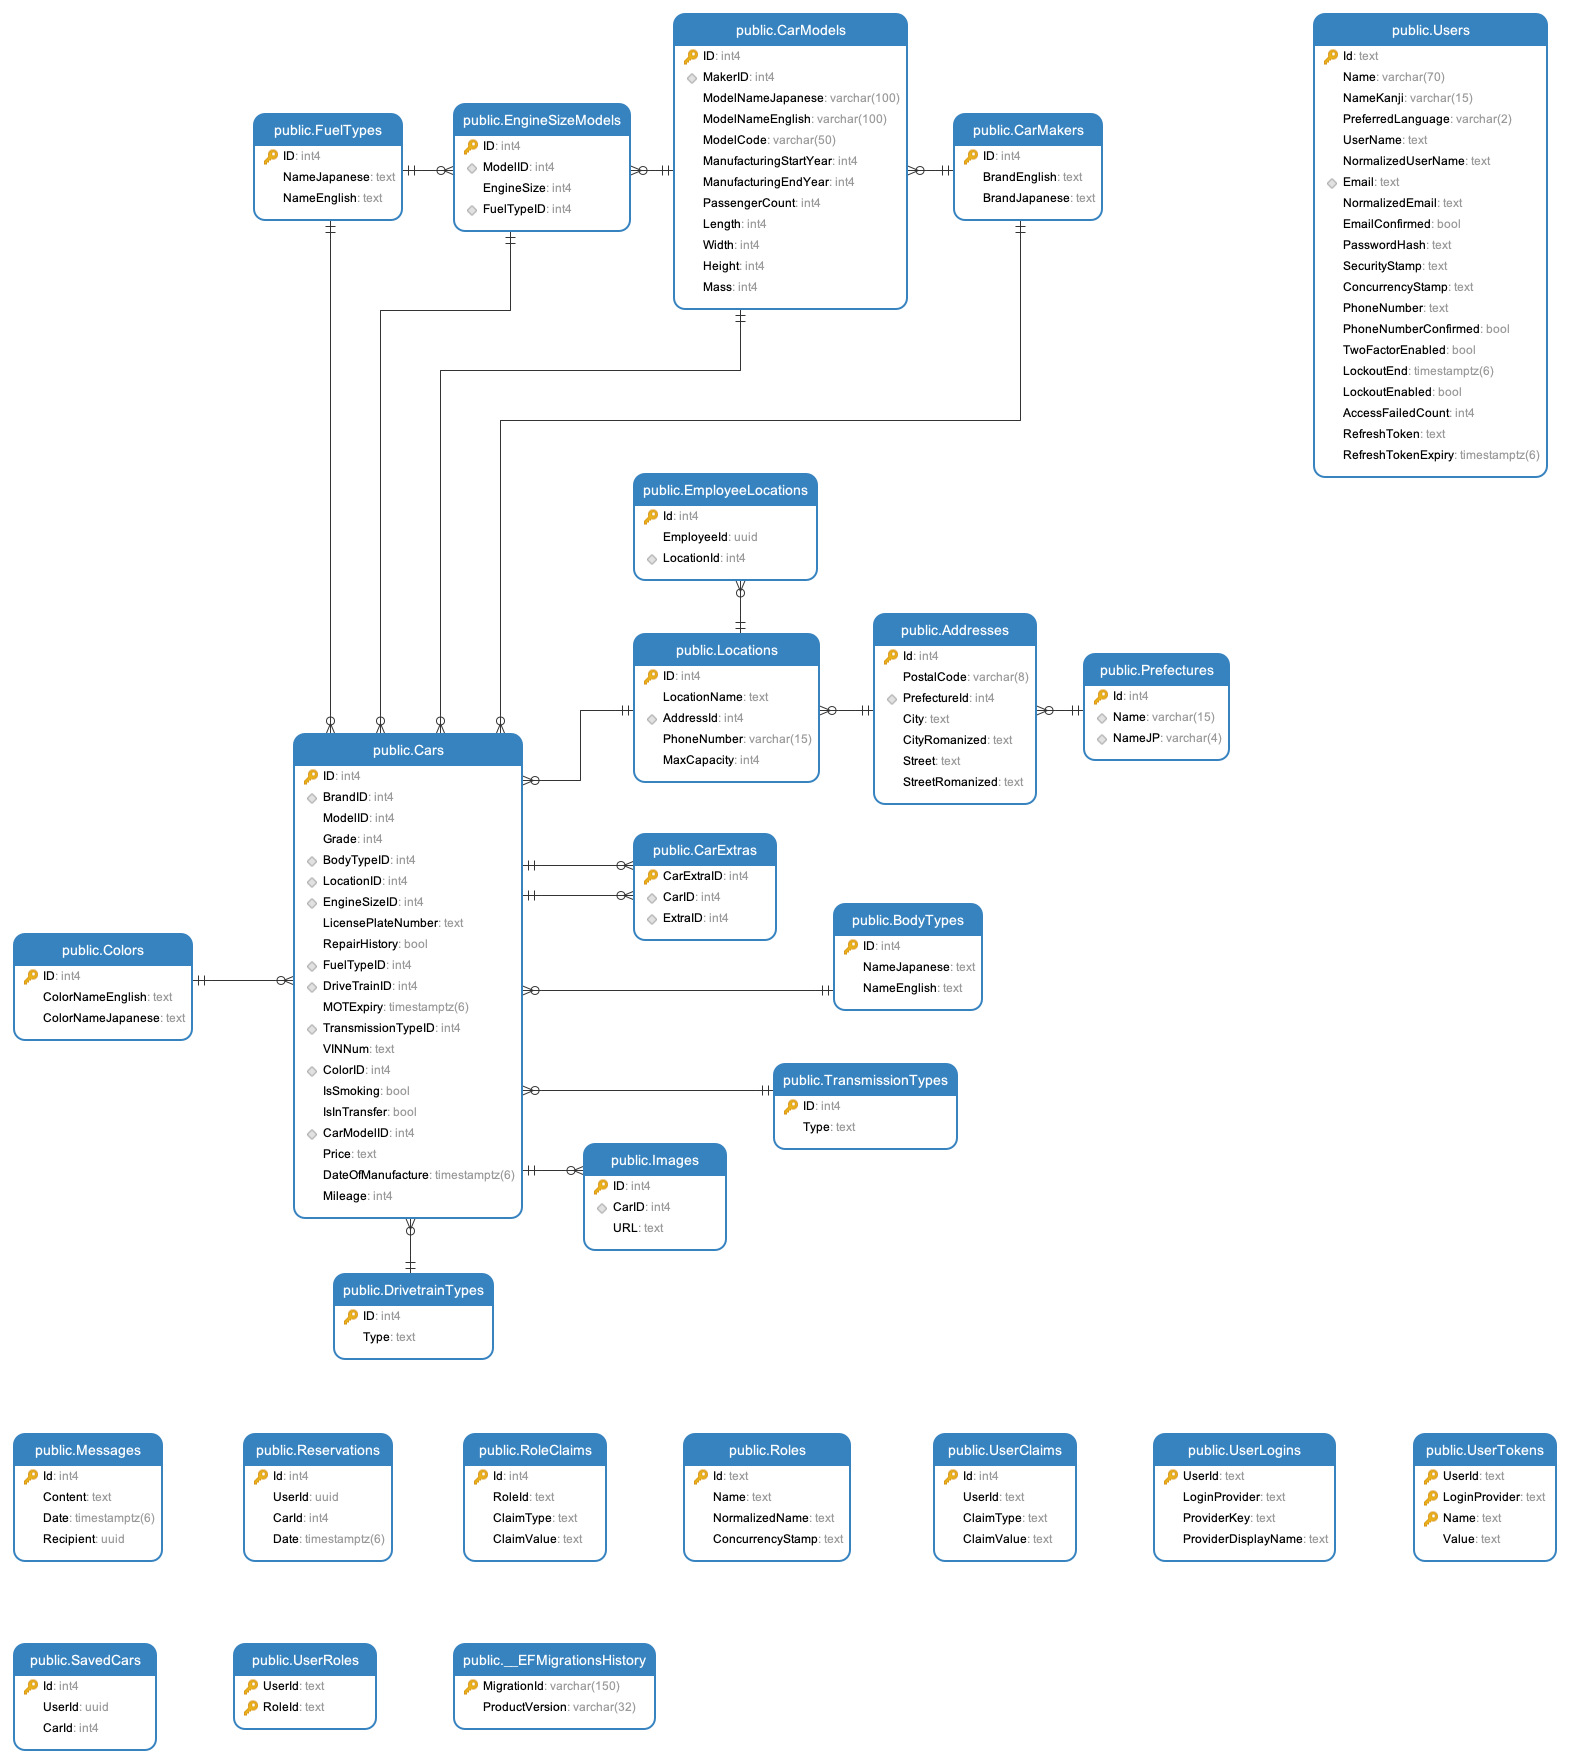
\includegraphics[width=1.0\textwidth]{figures/db_diagram.png} 
    \caption{Az adatbázis sémája és az entitások közötti kapcsolatok}
    \label{fig:db_schema}
\end{figure}

A PostgreSQL mellett való döntés egyik fő oka az volt, hogy a MySQL használata során az Entity Framework MacOS-en furcsa hibákat produkált, amelyek megakadályozták a fejlesztést. Mivel a fejlesztői környezetben a Windows használata nem volt opció, alternatív megoldásra volt szükség. A PostgreSQL ezzel szemben stabilan működött, és semmilyen problémát nem okozott a fejlesztés során.  

Mivel az alkalmazás az Entity Framework-öt használja az adatbázis-kezeléshez, a háttérben futó adatbázismotor cseréje viszonylag egyszerű feladat lenne, ha a jövőben mégis szükség lenne rá. Az EF biztosítja a platformfüggetlen működést, lehetővé téve az adatbázis sémájának módosítását anélkül, hogy manuálisan kellene beavatkozni az adatbázisba.  

Az adatbázis minden egyes táblájának részletes definíciója a modellek között található meg. Az Entity Framework konfigurálja az adatbázis tábláit, és az inicializálási folyamat során bizonyos táblákat előzetesen feltölt az alapvető működéshez szükséges adatokkal. Például az üzemanyagtípusok (\texttt{FuelType}) és a prefektúrák (\texttt{Prefecture}) adatai az adatbázis inicializálásakor automatikusan bekerülnek.
Ezeket most nem szeretném részletesen kiemelni, hiszen az ApplicationDbContext megtekintésével könnyen fény derül hogy melyek tartalmaznak HasData()-t. 



\section{Fájlstruktúra}

A projekt mappastruktúrája az alábbiak szerint van felépítve:

\subsection{Root könyvtár}
A projekt gyökérkönyvtárában találhatóak a projekt legfontosabb fájljai és beállításai:

\begin{itemize}
    \item \textbf{Program.cs}: Az alkalmazás belépési pontja, ahol az indítás és konfigurálás történik.
    \item \textbf{appsettings.json}: Az alkalmazás globális konfigurációs fájlja, amely adatbázis-kapcsolatokat és egyéb beállításokat tartalmaz.
    \item \textbf{appsettings.Development.json}: Fejlesztési környezethez szükséges külön konfiguráció.
    \item \textbf{DealershipSystem.http}: A HTTP-kéréseket és válaszokat tartalmazó fájl.
\end{itemize}

\subsection{Dependencies}
A \texttt{Dependencies} mappa tartalmazza az alkalmazás által használt összes külső függőséget:

\begin{itemize}
    \item \textbf{Assemblies}: Az összes szükséges assembly a projekt működéséhez.
    \item \textbf{Analyzers}: Az alkalmazás által használt kód-elemző eszközök.
    \item \textbf{Packages}: A projekt által használt NuGet csomagok.
    \item \textbf{Frameworks}: A projekt által használt keretrendszerek és platformok.
\end{itemize}

\subsection{wwwroot}
A statikus fájlokat, mint például képeket és egyéb webes erőforrásokat tartalmazza. A példák a következő képeket tartalmazzák:

\begin{itemize}
    \item \texttt{037d874d-d51b-4914-ae53-a847cf749f0f\_9572469A30241026W00106.jpg}
    \item \texttt{f363231b-e785-456f-bf59-94c27958880e\_9572469A30241026W00107.jpg}
\end{itemize}

\subsection{Configurations}
Ez a mappa tartalmazza az alkalmazás konfigurációs fájljait:

\begin{itemize}
    \item \textbf{PrefectureConfiguration.cs}: A prefektúrákkal kapcsolatos konfigurációk.
\end{itemize}

\subsection{Context}
Ez a mappa az adatbázis-kapcsolatok kezeléséért felelős fájlokat tartalmazza:

\begin{itemize}
    \item \textbf{ApplicationDbContext.cs}: Az adatbázis inicializálását és konfigurálását végző fájl.
\end{itemize}

\subsection{Controllers}

A vezérlők felelősek a HTTP-kérések kezeléséért, valamint az üzleti logika irányításáért. Az alábbi vezérlők találhatók a projektben:

\begin{itemize}
    \item \textbf{CarController.cs}: A járművekkel kapcsolatos kéréseket kezeli, mint például a járművek lekérése, létrehozása, frissítése és törlése.
    \item \textbf{CarMakerController.cs}: A járműgyártókkal kapcsolatos kéréseket kezeli, beleértve a gyártók listázását, hozzáadását és törlését.
    \item \textbf{CarMetadataController.cs}: A járművek metaadataival kapcsolatos műveleteket kezeli, például a kiegészítő adatok és paraméterek kezelését.
    \item \textbf{CarModelController.cs}: A járműmodellekhez tartozó kéréseket kezeli, mint a modellek listázása, hozzáadása és módosítása.
    \item \textbf{EmployeeLocationController.cs}: A dolgozói helyekkel kapcsolatos műveleteket kezeli, például a dolgozók helyeinek frissítését és kezelését.
    \item \textbf{EngineController.cs}: A motorokkal kapcsolatos kéréseket kezeli, például a motorok típusainak és paramétereinek lekérdezését és frissítését.
    \item \textbf{ImageController.cs}: A képekkel kapcsolatos műveleteket kezeli, például a képek feltöltését és lekérését a járművekhez.
    \item \textbf{LocationController.cs}: A helyekkel kapcsolatos kéréseket kezeli, mint például a helyek listázása, hozzáadása és törlése.
    \item \textbf{MessageController.cs}: Az üzenetkezeléssel kapcsolatos műveleteket kezeli, például üzenetek küldését és fogadását.
    \item \textbf{ReservationController.cs}: A foglalásokkal kapcsolatos kéréseket kezeli, például foglalások létrehozását, módosítását és törlését.
    \item \textbf{SavedCarsController.cs}: A mentett járművekkel kapcsolatos műveleteket kezeli, például járművek mentését és törlését.
    \item \textbf{UserController.cs}: A felhasználókkal kapcsolatos kéréseket kezeli, mint például felhasználói adatok lekérése, regisztráció és bejelentkezés.
\end{itemize}


\subsection{DTO}
A Data Transfer Object (DTO) osztályok az adatokat hordozzák az alkalmazás különböző rétegei között:

\begin{itemize}
    \item \textbf{AddressDTO.cs}: Címadatokat tartalmazó DTO.
    \item \textbf{AdminUserCreateDTO.cs}: Adminisztrátori felhasználó létrehozását tartalmazó DTO.
    \item \textbf{AdminUserUpdateDTO.cs}: Adminisztrátori felhasználó frissítését tartalmazó DTO.
    \item \textbf{BodyTypeDTO.cs}: Karosszériatípus adatokat tartalmazó DTO.
    \item \textbf{CarDTO.cs}: Járműadatokat tartalmazó DTO.
    \item \textbf{CarExtraDTO.cs}: Jármű extrák adatokat tartalmazó DTO.
    \item \textbf{CarMakerDTO.cs}: Járműgyártó adatokat tartalmazó DTO.
    \item \textbf{CarModelDTO.cs}: Járműmodell adatokat tartalmazó DTO.
    \item \textbf{ChangePasswordAdminDTO.cs}: Adminisztrátori jelszó módosítását tartalmazó DTO.
    \item \textbf{ChangePasswordDTO.cs}: Felhasználói jelszó módosítását tartalmazó DTO.
    \item \textbf{ColorDTO.cs}: Színadatokat tartalmazó DTO.
    \item \textbf{CreateBodyTypeDTO.cs}: Új karosszériatípus létrehozását tartalmazó DTO.
    \item \textbf{CreateCarDTO.cs}: Új jármű létrehozását tartalmazó DTO.
    \item \textbf{CreateCarMakerDTO.cs}: Új járműgyártó létrehozását tartalmazó DTO.
    \item \textbf{CreateCarModelDTO.cs}: Új járműmodell létrehozását tartalmazó DTO.
    \item \textbf{CreateEngineDTO.cs}: Új motor létrehozását tartalmazó DTO.
    \item \textbf{CreateReservationDTO.cs}: Új foglalás létrehozását tartalmazó DTO.
    \item \textbf{DealerLoginResponseDTO.cs}: Kereskedői bejelentkezés válaszát tartalmazó DTO.
    \item \textbf{DealerUserDTO.cs}: Kereskedői felhasználói adatokat tartalmazó DTO.
    \item \textbf{DrivetrainTypeDTO.cs}: Hajtáslánc típusokat tartalmazó DTO.
    \item \textbf{EngineSizeModelDTO.cs}: Motor méretmodellek adatokat tartalmazó DTO.
    \item \textbf{ExtraDTO.cs}: Jármű extrák általános adatokat tartalmazó DTO.
    \item \textbf{ExtraTypeDTO.cs}: Extra típusokat tartalmazó DTO.
    \item \textbf{FuelTypeDTO.cs}: Üzemanyagtípus adatokat tartalmazó DTO.
    \item \textbf{ImageDTO.cs}: Képadatokat tartalmazó DTO.
    \item \textbf{ImageUploadDTO.cs}: Képfeltöltési adatokat tartalmazó DTO.
    \item \textbf{LocationDTO.cs}: Helyadatokat tartalmazó DTO.
    \item \textbf{MessageDTO.cs}: Üzenetadatokat tartalmazó DTO.
    \item \textbf{PrefectureDTO.cs}: Prefektúra adatokat tartalmazó DTO.
    \item \textbf{ReservationDTO.cs}: Foglalási adatokat tartalmazó DTO.
    \item \textbf{TransmissionTypeDTO.cs}: Sebességváltó típusokat tartalmazó DTO.
    \item \textbf{UpdateCarMakerDTO.cs}: Járműgyártó frissítését tartalmazó DTO.
    \item \textbf{UpdateCarModelDTO.cs}: Járműmodell frissítését tartalmazó DTO.
    \item \textbf{UpdateEngineDTO.cs}: Motor frissítését tartalmazó DTO.
    \item \textbf{UpdateReservationDTO.cs}: Foglalás frissítését tartalmazó DTO.
    \item \textbf{UserDTO.cs}: Felhasználói adatokat tartalmazó DTO.
    \item \textbf{UserLoginDTO.cs}: Felhasználói bejelentkezési adatokat tartalmazó DTO.
    \item \textbf{UserRegisterDTO.cs}: Felhasználói regisztrációs adatokat tartalmazó DTO.
\end{itemize}

\subsection{Helpers}
Ez a mappa segédosztályokat tartalmaz, amelyek az alkalmazás különböző aspektusait segítik:

\begin{itemize}
    \item \textbf{AuthSettings.cs}: Az alkalmazás hitelesítési beállításait tartalmazó fájl.
    \item \textbf{SeedRoles.cs}: Az IdentityRole-hoz a szerepkörök feltőltése
\end{itemize}

\subsection{Interfaces}
A projekt interfészeit tartalmazó fájlok, amelyek a szolgáltatások közötti kommunikációt biztosítják:

\begin{itemize}
    \item \textbf{ICarMakerService.cs}: Járműgyártó szolgáltatás interfésze.
    \item \textbf{ICarModelService.cs}: Járműmodell szolgáltatás interfésze.
    \item \textbf{IEngineSizeModelService.cs}: Motorméret-modellek kezelési interfésze.
    \item \textbf{IMessageService.cs}: Üzenetek kezelési interfésze.
    \item \textbf{IReservationService.cs}: Foglalások kezelési interfésze.
    \item \textbf{ISavedCarService.cs}: Mentett járművek kezelési interfésze.
    \item \textbf{IUserService.cs}: Felhasználói szolgáltatás interfésze.
\end{itemize}

\subsection{Mappings}
A \texttt{MappingProfile.cs} fájl tartalmazza az összes adatátviteli mappa (DTO) és az adatmodellek közötti leképezéseket.

\subsection{Migrations}
A migrációs fájlokat tartalmazó mappa, amelyek lehetővé teszik az adatbázis sémájának módosítását. Ez az EntityFramework-höz tartozik.

\subsection{Models}
A projekt adatmodelljei, amelyek az adatbázis entitásait képviselik:

\begin{itemize}
    \item \textbf{Address.cs}: A cím adatmodellje, amely a cím adatait tárolja, beleértve a postal kódot, prefektúrát, várost és utcát.

    \begin{itemize}
        \item \textbf{Id}: A cím egyedi azonosítója.
        \item \textbf{PostalCode}: A címhez tartozó irányítószám. (Max 8 karakter hosszú)
        \item \textbf{PrefectureId}: A címhez tartozó prefektúra azonosítója.
        \item \textbf{Prefecture}: A címhez tartozó prefektúra (navigációs tulajdonság).
        \item \textbf{City}: A város neve japánul.
        \item \textbf{CityRomanized}: A város neve romanizált (latin betűs) formában.
        \item \textbf{Street}: Az utca neve.
        \item \textbf{StreetRomanized}: Az utca neve romanizált formában.
    \end{itemize}

    \item \textbf{BodyType.cs}: A jármű karosszéria típusát tároló adatmodell. Ez első migrációnál automatikusan feltöltődik az adatbázisba.

    \begin{itemize}
        \item \textbf{ID}: A karosszéria típus egyedi azonosítója. (Kötelező)
        \item \textbf{NameJapanese}: A karosszéria típus neve japánul.
        \item \textbf{NameEnglish}: A karosszéria típus neve angolul.
    \end{itemize}
    
    \item \textbf{Car.cs}: Jármű adatmodellje.

\begin{itemize}
    \item \textbf{ID}: A jármű egyedi azonosítója (primary key).
    \item \textbf{BrandID}: A jármű gyártójának azonosítója.
    \item \textbf{ModelID}: A jármű modelljének azonosítója.
    \item \textbf{Grade}: A jármű besorolása.
    \item \textbf{BodyTypeID}: A jármű karosszéria típusának azonosítója.
    \item \textbf{LocationID}: A jármű helyének azonosítója.
    \item \textbf{EngineSizeID}: A jármű motor méretének azonosítója.
    \item \textbf{LicensePlateNumber}: A jármű rendszáma.
    \item \textbf{RepairHistory}: A jármű javítási előzményeinek megléte.
    \item \textbf{FuelTypeID}: A jármű üzemanyag típusának azonosítója.
    \item \textbf{DriveTrainID}: A jármű hajtásláncának azonosítója.
    \item \textbf{MOTExpiry}: A jármű műszaki vizsgájának lejárata.
    \item \textbf{TransmissionTypeID}: A jármű váltójának típusának azonosítója.
    \item \textbf{VINNum}: A jármű alvázszáma (VIN).
    \item \textbf{ColorID}: A jármű színének azonosítója.
    \item \textbf{IsSmoking}: A jármű dohányzástól mentes-e.
    \item \textbf{Mileage}: A jármű futásteljesítménye.
    \item \textbf{IsInTransfer}: A jármű telephely közötti mozgatásban van-e. 
    \item \textbf{Price}: A jármű ára.

    \item \textbf{Navigation Properties}:
    \begin{itemize}
        \item \textbf{Brand}: A jármű gyártója (CarMaker).
        \item \textbf{CarModel}: A jármű modellje (CarModel).
        \item \textbf{BodyType}: A jármű karosszéria típusa (BodyType).
        \item \textbf{Location}: A jármű helye (Location).
        \item \textbf{EngineSize}: A jármű motorjának mérete (EngineSizeModel).
        \item \textbf{FuelType}: A jármű üzemanyagtípusa (FuelType).
        \item \textbf{DriveTrain}: A jármű hajtáslánca (DrivetrainType).
        \item \textbf{TransmissionType}: A jármű váltó típusa (TransmissionType).
        \item \textbf{Color}: A jármű színe (Color).
        \item \textbf{CarExtras}: A jármű extra felszereltségei (CarExtra).
        \item \textbf{Images}: A járműhöz tartozó képek (Image).
    \end{itemize}
    \item \textbf{DateOfManufacture}: A jármű gyártási dátuma.
\end{itemize}

    \item \textbf{CarExtra.cs}: Jármű extrák összekapcsolását biztosító adatmodell. Jelenleg nincs implementálva.\item 
    
    \textbf{CarMaker.cs}: A járműgyártót tároló adatmodell.

    \begin{itemize}
        \item \textbf{ID}: A járműgyártó egyedi azonosítója.
        \item \textbf{BrandEnglish}: A járműgyártó neve angolul.
        \item \textbf{BrandJapanese}: A járműgyártó neve japánul.
    \end{itemize}

\begin{itemize}
    \item \textbf{ID}: A gyártó azonosítója.
    \item \textbf{BrandEnglish}: A gyártó neve angol nyelven.
    \item \textbf{BrandJapanese}: A gyártó neve japán nyelven.
\end{itemize}
\item \textbf{Color.cs}: A színadatokat tároló adatmodell.

\begin{itemize}
    \item \textbf{ID}: A szín egyedi azonosítója (primary key).
    \item \textbf{ColorNameEnglish}: A szín neve angolul.
    \item \textbf{ColorNameJapanese}: A szín neve japánul.
    \item \textbf{Cars}: Kapcsolódó járművek gyűjteménye (Navigation property), amelyek a színhez tartoznak.
\end{itemize}

\item \textbf{EmployeeLocation.cs}: Alkalmazott helyadatmodellje.

\begin{itemize}
    \item \textbf{Id}: Az alkalmazott helyének egyedi azonosítója (primary key).
    \item \textbf{EmployeeId}: Az alkalmazott azonosítója (GUID, a felhasználói azonosító, amely a string típusú IdentityUser-tól származik).
    \item \textbf{LocationId}: Az alkalmazott hely azonosítója (külső kulcs a Location táblára).
    \item \textbf{Navigation Property}:
    \begin{itemize}
        \item \textbf{Location}: Az alkalmazott helye (Location). A hely a \textbf{LocationId} segítségével van kapcsolva.
    \end{itemize}
\end{itemize}

\item \textbf{EngineSizeModel.cs}: Motor méret modell adatmodellje.

\begin{itemize}
    \item \textbf{ID}: A motor méret modell egyedi azonosítója (primary key).
    \item \textbf{ModelID}: A kapcsolódó járműmodell azonosítója (külső kulcs a CarModel táblára).
    \item \textbf{EngineSize}: A motor mérete (300 és 10000 között, érvénytelen méret esetén hibát jelez).
    \item \textbf{Navigation Properties}:
    \begin{itemize}
        \item \textbf{FuelType}: A motor üzemanyag típusa.
        \item \textbf{CarModel}: A járműmodell, amelyhez a motor méret tartozik (a \textbf{ModelID} segítségével kapcsolódik). Az \textbf{JsonIgnore} attribútum miatt nem kerül bele a JSON-ba.
    \end{itemize}

\end{itemize}
\item \textbf{Extra.cs}: Az extra típusokat és azok nevét tároló adatmodell, amely kapcsolódik az \textbf{ExtraType} táblához.
\item \textbf{FuelType.cs}: Járművek üzemanyag típusait tároló adatmodell, mely előre be van töltve az adatbázisba.
\begin{itemize}
    \item \textbf{ID}: Az üzemanyag típus egyedi azonosítója (primary key).
    \item \textbf{NameJapanese}: Az üzemanyag típus neve japánul.
    \item \textbf{NameEnglish}: Az üzemanyag típus neve angolul.
\end{itemize}


\item \textbf{Grade.cs}: A járművek osztályozására szolgáló enumeráció.
\begin{itemize}
    \item \textbf{A}: Legjobb minőség.
    \item \textbf{B}: Kiváló minőség.
    \item \textbf{C}: Jó minőség.
    \item \textbf{D}: Megfelelő minőség.
    \item \textbf{E}: Elégtelen minőség.
\end{itemize}

\item \textbf{Image.cs}: Kép adatmodell, amely a járműhöz tartozó képeket tárolja.
\begin{itemize}
    \item \textbf{ID}: A kép egyedi azonosítója (primary key).
    \item \textbf{CarID}: A kapcsolódó jármű egyedi azonosítója (külső kulcs).
    \item \textbf{URL}: A kép elérhetősége (URL).
    \item \textbf{Car}: A kapcsolódó jármű.
\end{itemize}

\item \textbf{Location.cs}: A helyszín adatmodell, amely tartalmazza a helyszín nevét, címét és egyéb részleteit.
\begin{itemize}
    \item \textbf{ID}: A helyszín egyedi azonosítója (primary key).
    \item \textbf{LocationName}: A helyszín neve.
    \item \textbf{AddressId}: A kapcsolódó cím egyedi azonosítója (külső kulcs).
    \item \textbf{Address}: A helyszín címét tároló adatmodell.
    \item \textbf{MaxCapacity}: A helyszín maximális kapacitása.
    \item \textbf{PhoneNumber}: A helyszín telefonszáma.
\end{itemize}

\item \textbf{Message.cs}: Üzenet adatmodell, amely az üzenetek tartalmát, dátumát és címzettjét tartalmazza.
\begin{itemize}
    \item \textbf{Id}: Az üzenet egyedi azonosítója.
    \item \textbf{Content}: Az üzenet tartalma.
    \item \textbf{Date}: Az üzenet dátuma.
    \item \textbf{Recipient}: A címzett GUID azonosítója.
\end{itemize}

\item \textbf{Prefecture.cs}: Prefektúra adatmodell, amely Japán 47 prefektúráját tartalmazza.
\begin{itemize}
    \item \textbf{Id}: A prefektúra egyedi azonosítója (primary key).
    \item \textbf{Name}: A prefektúra neve.
    \item \textbf{NameJP}: A prefektúra neve japánul.
\end{itemize}

\item \textbf{Reservation.cs}: Foglalás adatmodell, amely tartalmazza a járműhöz kapcsolódó foglalásokat.
\begin{itemize}
    \item \textbf{Id}: A foglalás egyedi azonosítója.
    \item \textbf{UserId}: A felhasználó azonosítója, aki a foglalást tette.
    \item \textbf{CarId}: A foglalt jármű azonosítója.
    \item \textbf{Date}: A foglalás dátuma.
\end{itemize}

\item \textbf{SavedCar.cs}: Jármű mentési adatmodell, amely tárolja a felhasználók által mentett járműveket.
\begin{itemize}
    \item \textbf{Id}: A mentett jármű egyedi azonosítója.
    \item \textbf{UserId}: A felhasználó azonosítója, aki a járművet mentette.
    \item \textbf{CarId}: A mentett jármű azonosítója.
\end{itemize}

\item \textbf{TransmissionType.cs}: A járművek sebességváltó típusait tároló adatmodell.
\begin{itemize}
    \item \textbf{ID}: A sebességváltó típus egyedi azonosítója.
    \item \textbf{Type}: A sebességváltó típusa (pl. kézi, automatikus).
\end{itemize}

\item \textbf{User.cs}: Felhasználó adatmodell, amely az IdentityUser kiterjesztéseként tárolja a felhasználói adatokat.
\begin{itemize}
    \item \textbf{Name}: A felhasználó neve.
    \item \textbf{NameKanji}: A felhasználó neve kanjival (ha van).
    \item \textbf{PreferredLanguage}: A felhasználó preferált nyelve.
    \item \textbf{RefreshToken}: A felhasználó frissítő tokenje.
    \item \textbf{RefreshTokenExpiry}: A frissítő token lejárati ideje.
\end{itemize}
\end{itemize}

\subsection{Services}
Szolgáltatások, amelyek az alkalmazás üzleti logikáját tartalmazzák:

\begin{itemize}
    \item \textbf{CarMakerService.cs}: Járműgyártók kezelésére szolgáló osztály, amely lehetővé teszi a gyártók létrehozását, lekérését, frissítését és törlését. Az AutoMapper könyvtár segítségével biztosítja az adatok átvitelét a modellek és DTO-k között. 
    \item \textbf{CarMakerService.cs}: Járműgyártókkal kapcsolatos üzleti logika.
    \item \textbf{UserService.cs}: Felhasználókkal kapcsolatos üzleti logika.
    \item \textbf{ReservationService.cs}: Foglalásokkal kapcsolatos üzleti logika.
    \begin{figure}[h!]
        \centering
        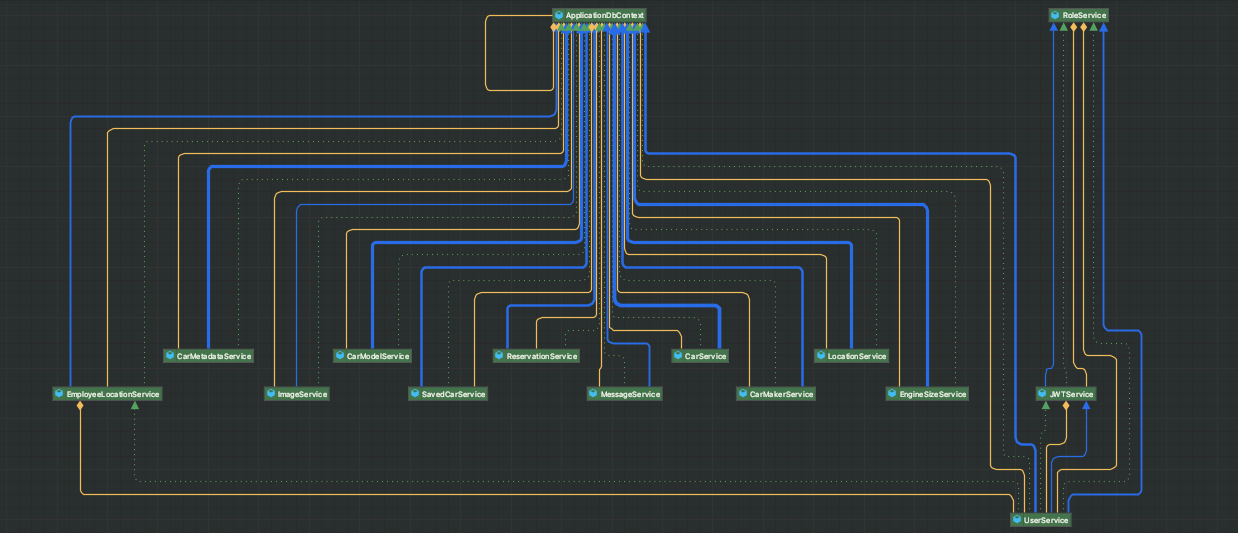
\includegraphics[width=\textwidth]{figures/class_dependencies.png} 
        \caption{A diagram a szolgáltatások közötti osztályfüggőségek ábrázolásáról.}
        \label{fig:classDependencies}
    \end{figure}    
\end{itemize}


\section{Osztályok}

\subsection{CarMakerService osztály}

Az \texttt{CarMakerService} osztály felelős a járműgyártók kezeléséért. Ez az osztály az alábbi funkciókat biztosítja:

\begin{itemize}
    \item \textbf{CreateNewMakerAsync}: Új autógyártó létrehozása, ha még nem létezik. Az adatok a DTO (Data Transfer Object) és az entitás között történő átvitelét az AutoMapper könyvtár biztosítja.
    \item \textbf{GetMakersAsync}: Az összes autógyártó lekérése.
    \item \textbf{GetMakerByIdAsync}: Az autógyártó lekérése ID alapján.
    \item \textbf{UpdateMakerByIdAsync}: Egy meglévő autógyártó frissítése ID alapján.
    \item \textbf{DeleteMakerByIdAsync}: Autógyártó törlése ID alapján.
\end{itemize}


Az osztály metódusai alább találhatók C\# kóddal és kommentekkel:

\subsection{CarMakerService implementációja}

\subsection*{CreateNewMakerAsync metódus}
\begin{lstlisting}
    /// <summary>
    /// Creates a new car maker in the database if it doesn't already exist.
    /// If the maker already exists, returns null.
    /// </summary>
    /// <param name="createCarMakerDto">The DTO containing car maker data to create.</param>
    /// <returns>A CarMakerDTO if creation was successful, or null if the maker already exists.</returns>
    public async Task<CarMakerDTO?> CreateNewMakerAsync(CreateCarMakerDTO createCarMakerDto)
\end{lstlisting}

\subsection*{GetMakersAsync metódus}
\begin{lstlisting}
    /// <summary>
    /// Retrieves all car makers from the database.
    /// </summary>
    /// <returns>A list of CarMakerDTOs representing all car makers.</returns>
    public async Task<List<CarMakerDTO>> GetMakersAsync()
\end{lstlisting}

\subsection*{GetMakerByIdAsync metódus}
\begin{lstlisting}
    /// <summary>
    /// Retrieves a specific car maker by its ID.
    /// </summary>
    /// <param name="id">The ID of the car maker to retrieve.</param>
    /// <returns>A CarMakerDTO representing the car maker, or null if not found.</returns>
    public async Task<CarMakerDTO?> GetMakerByIdAsync(int id)
\end{lstlisting}

\subsection*{UpdateMakerByIdAsync metódus}
\begin{lstlisting}
    /// <summary>
    /// Updates an existing car maker's data in the database by its ID.
    /// </summary>
    /// <param name="updateCarMakerDto">The DTO containing the updated car maker data.</param>
    /// <returns>The updated CarMakerDTO, or null if the maker was not found.</returns>
    public async Task<CarMakerDTO?> UpdateMakerByIdAsync(UpdateCarMakerDTO updateCarMakerDto)
\end{lstlisting}

\subsection*{DeleteMakerByIdAsync metódus}
\begin{lstlisting}
    /// <summary>
    /// Deletes a car maker by its ID from the database.
    /// </summary>
    /// <param name="id">The ID of the car maker to delete.</param>
    /// <returns>True if deletion was successful, false if the maker was not found.</returns>
    public async Task<bool> DeleteMakerByIdAsync(int id)
\end{lstlisting}

\subsection*{Összegzés}
A \texttt{CarMakerService} osztály egy átfogó megoldást kínál az autógyártók kezelésére, lehetővé téve a felhasználók számára, hogy könnyedén létrehozzanak, lekérdezzenek, frissítsenek és töröljenek autógyártókat. Az AutoMapper könyvtár használatával az adatok átvitele a DTO-k és az entitások között hatékonyan történik, biztosítva a tiszta és karbantartható kódot.



\subsection{CarMetadataService osztály}

Az \texttt{CarMetadataService} osztály felelős a járművek különböző metaadatai, mint például a karosszéria típusok, sebességváltó típusok, üzemanyag típusok, hajtáslánc típusok és színek kezeléséért. Az osztály az alábbi funkciókat biztosítja:

\begin{itemize}
    \item \textbf{CarMetadataService.cs}: Járműmetaadatok kezelésére szolgáló osztály, amely lehetővé teszi a karosszéria típusok, sebességváltó típusok, üzemanyag típusok, hajtáslánc típusok és színek létrehozását, lekérését.
    \item \textbf{CreateCarBodyTypeAsync}: Új karosszéria típus létrehozása, ha még nem létezik. Az adatok a DTO (Data Transfer Object) és az entitás között történő átvitelét az AutoMapper könyvtár biztosítja.
    \item \textbf{GetBodyTypesAsync}: Az összes karosszéria típus lekérése.
    \item \textbf{GetBodyTypeByIdAsync}: A karosszéria típusok lekérése ID alapján.
    \item \textbf{GetTransmissionTypesAsync}: Az összes sebességváltó típus lekérése.
    \item \textbf{GetTransmissionTypeByIdAsync}: Sebességváltó típus lekérése ID alapján.
    \item \textbf{GetFuelTypesAsync}: Az összes üzemanyag típus lekérése.
    \item \textbf{GetFuelTypeByIdAsync}: Üzemanyag típus lekérése ID alapján.
    \item \textbf{GetDrivetrainTypesAsync}: Az összes hajtáslánc típus lekérése.
    \item \textbf{GetDrivetrainTypeByIdAsync}: Hajtáslánc típus lekérése ID alapján.
    \item \textbf{GetColorTypesAsync}: Az összes szín típus lekérése.
    \item \textbf{GetColorByIdAsync}: Szín típus lekérése ID alapján.
\end{itemize}

\subsection{CarMakerService implementációja}

\subsection*{CreateCarBodyTypeAsync Metódus}
\begin{lstlisting}
    /// <summary>
    /// Creates a new car body type if it does not already exist.
    /// </summary>
    /// <param name="bodyTypeDto">The DTO containing body type details.</param>
    /// <returns>A tuple containing the body type entity and a boolean indicating if it was newly created.</returns>
    public async Task<(BodyType bodyType, bool isNew)> CreateCarBodyTypeAsync(CreateBodyTypeDTO bodyTypeDto)
\end{lstlisting}


\subsection*{GetBodyTypesAsync Metódus}
\begin{lstlisting}
    /// <summary>
    /// Retrieves a list of all body types.
    /// </summary>
    /// <returns>A list of body type DTOs.</returns>
    public async Task<List<BodyTypeDTO>> GetBodyTypesAsync()
\end{lstlisting}

\subsection*{GetBodyTypeByIdAsync Metódus}
\begin{lstlisting}
    /// <summary>
    /// Retrieves a body type by its ID.
    /// </summary>
    /// <param name="id">The ID of the body type.</param>
    /// <returns>The body type DTO if found, otherwise null.</returns>
    public async Task<BodyTypeDTO?> GetBodyTypeByIdAsync(int id)
\end{lstlisting}

\subsection*{GetTransmissionTypesAsync Metódus}
\begin{lstlisting}
    /// <summary>
    /// Retrieves a list of all transmission types.
    /// </summary>
    /// <returns>A list of transmission type DTOs.</returns>
    public async Task<List<TransmissionTypeDTO>> GetTransmissionTypesAsync()
\end{lstlisting}

\subsection*{GetTransmissionTypeByIdAsync Metódus}
\begin{lstlisting}
    /// <summary>
    /// Retrieves a transmission type by its ID.
    /// </summary>
    /// <param name="id">The ID of the transmission type.</param>
    /// <returns>The transmission type DTO if found, otherwise null.</returns>
    public async Task<BodyTypeDTO?> GetTransmissionTypeByIdAsync(int id)
\end{lstlisting}

\subsection*{GetFuelTypesAsync Metódus}
\begin{lstlisting}
    /// <summary>
    /// Retrieves a list of all fuel types.
    /// </summary>
    /// <returns>A list of fuel type DTOs.</returns>
    public async Task<List<FuelTypeDTO>> GetFuelTypesAsync()
\end{lstlisting}

\subsection*{GetFuelTypeByIdAsync Metódus}
\begin{lstlisting}
    /// <summary>
    /// Retrieves a fuel type by its ID.
    /// </summary>
    /// <param name="id">The ID of the fuel type.</param>
    /// <returns>The fuel type DTO if found, otherwise null.</returns>
    public async Task<FuelTypeDTO?> GetFuelTypeByIdAsync(int id)
\end{lstlisting}

\subsection*{GetDrivetrainTypesAsync Metódus}
\begin{lstlisting}
    /// <summary>
    /// Retrieves a list of all drivetrain types.
    /// </summary>
    /// <returns>A list of drivetrain type DTOs.</returns>
    public async Task<List<DrivetrainTypeDTO>> GetDrivetrainTypesAsync()
\end{lstlisting}

\subsection*{GetDrivetrainTypeByIdAsync Metódus}
\begin{lstlisting}
    /// <summary>
    /// Retrieves a drivetrain type by its ID.
    /// </summary>
    /// <param name="id">The ID of the drivetrain type.</param>
    /// <returns>The drivetrain type DTO if found, otherwise null.</returns>
    public async Task<DrivetrainTypeDTO?> GetDrivetrainTypeByIdAsync(int id)
\end{lstlisting}

\subsection*{GetColorTypesAsync Metódus}
\begin{lstlisting}
    /// <summary>
    /// Retrieves a list of all color types.
    /// </summary>
    /// <returns>A list of color type DTOs.</returns>
    public async Task<List<ColorDTO>> GetColorTypesAsync()
\end{lstlisting}

\subsection*{GetColorByIdAsync Metódus}
\begin{lstlisting}
    /// <summary>
    /// Retrieves a color by its ID.
    /// </summary>
    /// <param name="id">The ID of the color.</param>
    /// <returns>The color DTO if found, otherwise null.</returns>
    public async Task<ColorDTO?> GetColorByIdAsync(int id)
\end{lstlisting}
\subsection*{Összegzés}
A \texttt{CarService} osztály egy átfogó megoldást kínál a járművek kezelésére, lehetővé téve a felhasználók számára, hogy könnyedén létrehozzanak, lekérdezzenek, frissítsenek és töröljenek járműveket. Az AutoMapper könyvtár használatával az adatok átvitele a DTO-k és az entitások között hatékonyan történik, biztosítva a tiszta és karbantartható kódot.

\subsection{CarModelService osztály}

Az \texttt{CarModelService} osztály felelős a járműmodellek kezeléséért, beleértve azok létrehozását, lekérését, frissítését és törlését. Az osztály az alábbi funkciókat biztosítja:

\begin{itemize}
    \item \textbf{CarModelService.cs}: Járműmodellek kezelésére szolgáló osztály, amely lehetővé teszi a járműmodellek létrehozását, lekérését, frissítését és törlését.
    \item \textbf{CreateCarModelAsync}: Új járműmodell létrehozása. Az adatok a DTO (Data Transfer Object) és az entitás között történő átvitelét az AutoMapper könyvtár biztosítja.
    \item \textbf{GetCarModelAsync}: Járműmodell lekérése ID alapján.
    \item \textbf{GetCarModelsFilteredAsync}: Járműmodellek lekérése opcionális paraméterek alapján.
    \item \textbf{GetAllCarModelsAsync}: Az összes járműmodell lekérése.
    \item \textbf{UpdateCarModelAsync}: Meglévő járműmodell frissítése.
    \item \textbf{DeleteCarModelAsync}: Járműmodell törlése ID alapján.
    \item \textbf{GetCarsByMakerIdAsync}: Járműmodellek lekérése a gyártó ID-ja alapján.
\end{itemize}

\subsection*{CreateCarModelAsync Metódus}
\begin{lstlisting}
    /// <summary>
    /// Creates a new car model.
    /// </summary>
    /// <param name="carModelDTO">The car model data transfer object.</param>
    /// <returns>The created CarModelDTO.</returns>
    public async Task<CarModelDTO> CreateCarModelAsync(CreateCarModelDTO carModelDTO)
\end{lstlisting}

\subsection*{GetCarModelAsync Metódus}
\begin{lstlisting}
    /// <summary>
    /// Retrieves a car model by its ID.
    /// </summary>
    /// <param name="id">The car model ID.</param>
    /// <returns>The CarModelDTO if found, otherwise null.</returns>
    public async Task<CarModelDTO?> GetCarModelAsync(int id)
\end{lstlisting}

\subsection*{GetCarModelsFilteredAsync Metódus}
\begin{lstlisting}
    /// <summary>
    /// Retrieves car models filtered by optional parameters.
    /// </summary>
    /// <param name="makerID">The maker ID to filter by.</param>
    /// <param name="startYear">The manufacturing start year to filter by.</param>
    /// <param name="endYear">The manufacturing end year to filter by.</param>
    /// <param name="passengerCount">The passenger count to filter by.</param>
    /// <returns>A list of filtered CarModelDTOs.</returns>
    public async Task<List<CarModelDTO>> GetCarModelsFilteredAsync(int? makerID = null, int? startYear = null, int? endYear = null,
        int? passengerCount = null)
\end{lstlisting}

\subsection*{GetAllCarModelsAsync Metódus}
\begin{lstlisting}
    /// <summary>
    /// Retrieves all car models.
    /// </summary>
    /// <returns>A list of CarModelDTOs.</returns>
    public async Task<List<CarModelDTO>> GetAllCarModelsAsync()
\end{lstlisting}

\subsection*{UpdateCarModelAsync Metódus}
\begin{lstlisting}
    /// <summary>
    /// Updates an existing car model.
    /// </summary>
    /// <param name="id">The ID of the car model to update.</param>
    /// <param name="updatedCarModel">The updated car model data.</param>
    /// <returns>The updated CarModelDTO, or null if not found.</returns>
    public async Task<CarModelDTO?> UpdateCarModelAsync(int id, UpdateCarModelDTO updatedCarModel)
\end{lstlisting}

\subsection*{DeleteCarModelAsync Metódus}
\begin{lstlisting}
    /// <summary>
    /// Deletes a car model by ID.
    /// </summary>
    /// <param name="id">The ID of the car model to delete.</param>
    /// <returns>True if deleted, false if not found.</returns>
    public async Task<bool> DeleteCarModelAsync(int id)
\end{lstlisting}

\subsection*{GetCarsByMakerIdAsync Metódus}
\begin{lstlisting}
    /// <summary>
    /// Retrieves all car models for a given maker ID.
    /// </summary>
    /// <param name="makerId">The maker ID.</param>
    /// <returns>A list of CarModelDTOs.</returns>
    public async Task<List<CarModelDTO>> GetCarsByMakerIdAsync(int makerId)
\end{lstlisting}
\subsection*{Összegzés}
A \texttt{CarModelService} osztály egy átfogó megoldást kínál a járműmodellek kezelésére, lehetővé téve a felhasználók számára, hogy könnyedén létrehozzanak, lekérdezzenek, frissítsenek és töröljenek járműmodelleket. Az AutoMapper könyvtár használatával az adatok átvitele a DTO-k és az entitások között hatékonyan történik, biztosítva a tiszta és karbantartható kódot.

\subsection{CarService osztály}

Az \texttt{CarService} osztály felelős a járművekkel kapcsolatos műveletek kezeléséért, beleértve a járművek lekérését, hozzáadását, frissítését és törlését. Az osztály az alábbi funkciókat biztosítja:

\begin{itemize}
    \item \textbf{CarService.cs}: Járművekkel kapcsolatos műveletek kezelésére szolgáló osztály, amely lehetővé teszi a járművek létrehozását, lekérését, frissítését és törlését.
    \item \textbf{GetAllCarsAsync}: Az összes jármű lekérése az adatbázisból.
    \item \textbf{GetCarByIdAsync}: Egy adott jármű lekérése ID alapján.
    \item \textbf{AddCarAsync}: Új jármű hozzáadása az adatbázishoz.
    \item \textbf{DeleteCarAsync}: Jármű törlése ID alapján.
    \item \textbf{EditCarAsync}: Meglévő járműadatok frissítése.
\end{itemize}

\subsection*{GetAllCarsAsync Metódus}
\begin{lstlisting}
    /// <summary>
    /// Retrieves all cars from the database.
    /// </summary>
    /// <returns>A list of CarDTOs.</returns>
    public async Task<List<CarDTO>> GetAllCarsAsync()
\end{lstlisting}

\subsection*{GetCarByIdAsync Metódus}
\begin{lstlisting}
    /// <summary>
    /// Retrieves a specific car by ID.
    /// </summary>
    /// <param name="id">The car ID.</param>
    /// <returns>The CarDTO if found, otherwise null.</returns>
    public async Task<CarDTO?> GetCarByIdAsync(int id)
\end{lstlisting}

\subsection*{AddCarAsync Metódus}
\begin{lstlisting}
    /// <summary>
    /// Adds a new car to the database.
    /// </summary>
    /// <param name="createCarDto">The car data to be added.</param>
    /// <returns>The created CarDTO.</returns>
    public async Task<CarDTO> AddCarAsync(CreateCarDTO createCarDto)
\end{lstlisting}

\subsection*{DeleteCarAsync Metódus}
\begin{lstlisting}
    /// <summary>
    /// Deletes a car from the database by ID.
    /// </summary>
    /// <param name="id">The ID of the car to delete.</param>
    /// <returns>True if deleted, false if not found.</returns>
    public async Task<bool> DeleteCarAsync(int id)
\end{lstlisting}

\subsection*{EditCarAsync Metódus}
\begin{lstlisting}
    /// <summary>
    /// Updates an existing car record.
    /// </summary>
    /// <param name="id">The ID of the car to update.</param>
    /// <param name="editCarDto">The updated car data.</param>
    /// <returns>The updated CarDTO, or null if not found.</returns>
    public async Task<CarDTO?> EditCarAsync(int id, CreateCarDTO editCarDto)
\end{lstlisting}

\subsection*{Összegzés}
A \texttt{CarService} osztály egy átfogó megoldást kínál a járművek kezelésére, lehetővé téve a felhasználók számára, hogy könnyedén létrehozzanak, lekérdezzenek, frissítsenek és töröljenek járműveket. Az AutoMapper könyvtár használatával az adatok átvitele a DTO-k és az entitások között hatékonyan történik, biztosítva a tiszta és karbantartható kódot.

\subsection{EmployeeLocationService osztály}

Az \texttt{EmployeeLocationService} osztály felelős az alkalmazottak helyszíneinek kezeléséért. Az osztály az alábbi funkciókat biztosítja:

\begin{itemize}
    \item \textbf{GetAllEmployeeLocationsAsync}: Az összes alkalmazott helyszínének lekérése az adatbázisból.
    \item \textbf{GetEmployeeLocationByEmployeeIdAsync}: Az alkalmazott helyszínének lekérése alkalmazott ID alapján.
    \item \textbf{AddEmployeeLocationAsync}: Új alkalmazott helyszín hozzáadása az adatbázishoz.
\end{itemize}

\subsection{EmployeeLocationService implementációja}

\subsection*{GetAllEmployeeLocationsAsync Metódus}
\begin{lstlisting}
    /// <summary>
    /// Retrieves all employee locations from the database.
    /// </summary>
    /// <returns>A list of employee locations.</returns>
    public async Task<List<EmployeeLocation>> GetAllEmployeeLocationsAsync()
\end{lstlisting}

\subsection*{GetEmployeeLocationByEmployeeIdAsync Metódus}
\begin{lstlisting}
    /// <summary>
    /// Retrieves an employee location by employee ID.
    /// </summary>
    /// <param name="employeeId">The employee ID.</param>
    /// <returns>The employee location if found, otherwise null.</returns>
    public async Task<EmployeeLocation?> GetEmployeeLocationByEmployeeIdAsync(Guid employeeId)
\end{lstlisting}

\subsection*{AddEmployeeLocationAsync Metódus}
\begin{lstlisting}
    /// <summary>
    /// Adds a new employee location to the database.
    /// </summary>
    /// <param name="employeeLocation">The employee location data to be added.</param>
    /// <returns>True if the operation was successful, otherwise false.</returns>
    public async Task<bool> AddEmployeeLocationAsync(EmployeeLocation employeeLocation)
\end{lstlisting}

\subsection*{Összegzés}
A \texttt{EmployeeLocationService} osztály egy átfogó megoldást kínál az alkalmazottak helyszíneinek kezelésére, lehetővé téve a felhasználók számára, hogy könnyedén lekérdezzék az alkalmazottak helyszíneit és új helyszíneket adjanak hozzá az adatbázishoz. Az aszinkron műveletek biztosítják, hogy az adatbázis lekérdezések és módosítások hatékonyan és gyorsan történjenek.

\subsection{EngineSizeService osztály}

Az \texttt{EngineSizeService} osztály felelős a motor méretek kezeléséért. Az osztály az alábbi funkciókat biztosítja:

\begin{itemize}
    \item \textbf{AddEngineSizeAsync}: Új motor méret hozzáadása az adatbázishoz.
    \item \textbf{GetEnginesAsync}: Az összes motor méret lekérése.
    \item \textbf{GetEngineByModelIdAsync}: Motor méretek lekérése autó modell ID alapján.
    \item \textbf{UpdateEngineAsync}: Egy meglévő motor méret frissítése.
    \item \textbf{DeleteEnginesAsync}: Motor méret törlése az adatbázisból.
\end{itemize}

\subsection{EngineSizeService implementációja}

\subsection*{AddEngineSizeAsync Metódus}
\begin{lstlisting}
    /// <summary>
    /// Adds a new engine size entry to the database.
    /// </summary>
    /// <param name="modelId">The ID of the car model.</param>
    /// <param name="engineSize">The engine size in cubic centimeters.</param>
    /// <param name="fuelTypeId">The ID of the fuel type.</param>
    /// <returns>The added engine size as a DTO.</returns>
    /// <exception cref="KeyNotFoundException">Thrown if the car model is not found.</exception>
    public async Task<EngineSizeModelDTO> AddEngineSizeAsync(int modelId, int engineSize, int fuelTypeId)
\end{lstlisting}

\subsection*{GetEnginesAsync Metódus}
\begin{lstlisting}
    /// <summary>
    /// Retrieves all engine sizes from the database.
    /// </summary>
    /// <returns>A list of engine size DTOs.</returns>
    public async Task<List<EngineSizeModelDTO>> GetEnginesAsync()
\end{lstlisting}

\subsection*{GetEngineByModelIdAsync Metódus}
\begin{lstlisting}
    /// <summary>
    /// Retrieves engine sizes by car model ID.
    /// </summary>
    /// <param name="modelId">The car model ID.</param>
    /// <returns>A collection of engine size DTOs, or null if none are found.</returns>
    public async Task<IEnumerable<EngineSizeModelDTO>?> GetEngineByModelIdAsync(int modelId)
\end{lstlisting}

\subsection*{UpdateEngineAsync Metódus}
\begin{lstlisting}
    /// <summary>
    /// Updates an existing engine size entry.
    /// </summary>
    /// <param name="engineId">The ID of the engine size entry.</param>
    /// <param name="newEngineSize">The updated engine size.</param>
    /// <param name="fuelTypeId">The new fuel type ID.</param>
    /// <returns>The updated engine size DTO if successful, otherwise null.</returns>
    public async Task<EngineSizeModelDTO?> UpdateEngineAsync(int engineId, int newEngineSize, int fuelTypeId)
\end{lstlisting}

\subsection*{DeleteEnginesAsync Metódus}
\begin{lstlisting}
    /// <summary>
    /// Deletes an engine size entry from the database.
    /// </summary>
    /// <param name="engineId">The ID of the engine size entry to delete.</param>
    /// <returns>True if deletion was successful, otherwise false.</returns>
    public async Task<bool> DeleteEnginesAsync(int engineId)
\end{lstlisting}

\subsection*{Összegzés}
A \texttt{EngineSizeService} osztály egy átfogó megoldást kínál a motor méretek kezelésére, lehetővé téve a felhasználók számára, hogy könnyedén hozzáadják, lekérdezzék, frissítsék és töröljék a motor méreteket az adatbázisból. Az AutoMapper könyvtár segítségével az adatok átvitele az entitások és DTO-k között hatékonyan és karbantartható módon történik. Az aszinkron műveletek biztosítják a magas teljesítményt és a hatékony adatkezelést.

\subsection{ImageService osztály}

Az \texttt{ImageService} osztály felelős a képek feltöltéséért és lekéréséért a járművekhez. Az osztály az alábbi funkciókat biztosítja:

\begin{itemize}
    \item \textbf{UploadImageAsync}: Kép feltöltése egy adott járműhöz.
    \item \textbf{GetImagesForCarAsync}: Az adott járműhöz tartozó összes kép URL-jének lekérése.
\end{itemize}

\subsection{ImageService implementációja}

\subsection*{UploadImageAsync Metódus}
\begin{lstlisting}
    /// <summary>
    /// Uploads an image for a specific car.
    /// </summary>
    /// <param name="imageFile">The image file to upload.</param>
    /// <param name="carId">The ID of the car associated with the image.</param>
    /// <returns>The URL of the uploaded image.</returns>
    /// <exception cref="ArgumentException">Thrown when the provided file is invalid.</exception>
    public async Task<string> UploadImageAsync(IFormFile imageFile, int carId)
\end{lstlisting}

\subsection*{GetImagesForCarAsync Metódus}
\begin{lstlisting}
    /// <summary>
    /// Retrieves all image URLs associated with a specific car.
    /// </summary>
    /// <param name="carId">The ID of the car.</param>
    /// <returns>A list of image URLs.</returns>
    public async Task<List<string>> GetImagesForCarAsync(int carId)
\end{lstlisting}

\subsection*{Összegzés}
A \texttt{ImageService} osztály lehetővé teszi a járművekhez tartozó képek kezelését. Az osztály biztosítja a képek feltöltését az adott járműhöz, a fájlok a szerveren a \texttt{wwwroot/uploads/{carId}} könyvtárban kerülnek tárolásra. Ha a kép már létezik, az URL visszaadásra kerül, anélkül hogy újra feltöltené. Az adatbázisban tárolja a kép URL-jét is. Az osztály emellett képes lekérni az adott járműhöz tartozó összes kép URL-jét.

\subsection{JWTService osztály}

A \texttt{JWTService} osztály felelős a JWT alapú hitelesítés kezeléséért. Az osztály biztosítja a felhasználói tokent generáló, a frissítő tokent generáló, és azok kezelését.

\begin{itemize}
    \item \textbf{GenerateTokens}: Generálja a hozzáférési és frissítő tokeneket egy felhasználó számára.
    \item \textbf{GenerateRefreshToken}: Biztonságos frissítő tokent generál.
    \item \textbf{RefreshAccessToken}: Frissíti a hozzáférési tokent egy érvényes frissítő token segítségével.
    \item \textbf{RevokeRefreshToken}: Érvényteleníti a frissítő tokent.
    \item \textbf{GenerateClaims}: Generálja a felhasználói azonosítókat és jogosultságokat.
\end{itemize}

\subsection{JWTService implementációja}

\subsection*{GenerateTokens Metódus}
\begin{lstlisting}
    /// <summary>
    /// Generates access and refresh tokens for a user.
    /// </summary>
    /// <param name="user">The user for whom the tokens are generated.</param>
    /// <returns>A tuple containing the access token and refresh token.</returns>
    public async Task<(string AccessToken, string RefreshToken)> GenerateTokens(User user)
\end{lstlisting}

\subsection*{GenerateRefreshToken Metódus}
\begin{lstlisting}
    /// <summary>
    /// Generates a secure refresh token.
    /// </summary>
    /// <returns>A base64-encoded refresh token.</returns>
    private string GenerateRefreshToken()
\end{lstlisting}

\subsection*{RefreshAccessToken Metódus}
\begin{lstlisting}
    /// <summary>
    /// Refreshes the access token using a valid refresh token.
    /// </summary>
    /// <param name="refreshToken">The refresh token.</param>
    /// <returns>A tuple indicating whether the operation was successful and the new access token.</returns>
    public async Task<(bool IsValid, string AccessToken)> RefreshAccessToken(string refreshToken)
\end{lstlisting}

\subsection*{RevokeRefreshToken Metódus}
\begin{lstlisting}
    /// <summary>
    /// Revokes a refresh token, making it invalid.
    /// </summary>
    /// <param name="refreshToken">The refresh token to revoke.</param>
    /// <returns>A boolean indicating whether the operation was successful.</returns>
    public async Task<bool> RevokeRefreshToken(string refreshToken)
\end{lstlisting}

\subsection*{GenerateClaims Metódus}
\begin{lstlisting}
    /// <summary>
    /// Generates claims for a user.
    /// </summary>
    /// <param name="user">The user whose claims are generated.</param>
    /// <returns>A ClaimsIdentity containing user claims.</returns>
    private async Task<ClaimsIdentity> GenerateClaims(User user)
\end{lstlisting}

\subsection*{Összegzés}
A \texttt{JWTService} osztály lehetővé teszi a felhasználók számára, hogy biztonságosan kezeljék a hozzáférési és frissítő tokeneket, amelyek szükségesek a felhasználók hitelesítéséhez és az API-hoz való hozzáféréshez. A frissítő tokenek 30 napig érvényesek, míg a hozzáférési tokenek 15 percig maradnak érvényben. Az osztály kezeli a frissítő tokenek visszavonását is, és biztosítja, hogy a felhasználói jogosultságok a megfelelő módon legyenek érvényesítve a JWT-k segítségével.

\subsection{MessageService osztály}

A \texttt{MessageService} osztály felelős az üzenetek kezeléséért a kereskedelmi rendszerben. Az osztály lehetővé teszi új üzenetek létrehozását, meglévő üzenetek lekérését és törlését.

\begin{itemize}
    \item \textbf{CreateMessageAsync}: Létrehozza az új üzenetet egy adott címzett számára.
    \item \textbf{GetMessagesByUserAsync}: Lekéri a felhasználó összes üzenetét.
    \item \textbf{DeleteMessageAsync}: Törli a megadott üzenetet.
    \item \textbf{GetUserIdFromJwt}: Kinyeri a felhasználó azonosítóját a JWT-ből.
\end{itemize}


\subsection{MessageService implementációja}

\subsection*{CreateMessageAsync Metódus}
\begin{lstlisting}
    /// <summary>
    /// Creates a new message asynchronously.
    /// </summary>
    /// <param name="content">The content of the message.</param>
    /// <param name="recipient">The recipient's ID.</param>
    public async Task CreateMessageAsync(string content, Guid recipient)
\end{lstlisting}

\subsection*{GetMessagesByUserAsync Metódus}
\begin{lstlisting}
    /// <summary>
    /// Gets messages by user ID asynchronously.
    /// </summary>
    /// <param name="userId">The user's ID.</param>
    /// <returns>A list of messages for the specified user.</returns>
    /// <exception cref="UnauthorizedAccessException">Thrown if the current user is not authorized to view the messages.</exception>
    public async Task<List<Message>> GetMessagesByUserAsync(Guid userId)
\end{lstlisting}

\subsection*{GetUserIdFromJwt Metódus}
\begin{lstlisting}
    /// <summary>
    /// Gets the user ID from the JWT.
    /// </summary>
    /// <returns>The user ID as a Guid.</returns>
    /// <exception cref="UnauthorizedAccessException">Thrown if the user ID is not found in the JWT.</exception>
    private Guid GetUserIdFromJwt()
\end{lstlisting}

\subsection*{DeleteMessageAsync Metódus}
\begin{lstlisting}
    /// <summary>
    /// Deletes a message asynchronously.
    /// </summary>
    /// <param name="messageId">The ID of the message to delete.</param>
    /// <exception cref="KeyNotFoundException">Thrown if the message is not found.</exception>
    /// <exception cref="UnauthorizedAccessException">Thrown if the current user is not authorized to delete the message.</exception>
    public async Task DeleteMessageAsync(int messageId)
\end{lstlisting}

\subsection*{Összegzés}
A \texttt{MessageService} osztály biztosítja az üzenetek kezelését a rendszerben. A felhasználók számára lehetőséget biztosít új üzenetek létrehozására, meglévő üzenetek lekérdezésére és törlésére. Az osztály a JWT-t használja a felhasználói azonosításra, és biztosítja, hogy csak a jogosult felhasználók férhessenek hozzá és törölhessenek üzeneteket. Az üzenetek törléséhez a felhasználónak először azonosítania kell magát, és biztosítani kell, hogy az üzenet neki legyen címzett.


\section{Bevezetés}
Ez a dokumentáció a \texttt{LocationServiceTests} osztály egységtesztjeit tartalmazza, amely a \texttt{DealershipSystem} rendszerben a helyszínekkel kapcsolatos funkciók teszteléséért felel. A tesztek az \texttt{xUnit}, \texttt{Moq} és \texttt{AutoMapper} keretrendszereket használják.

\section{Tesztkörnyezet}
\subsection{Használt technológiák}
\begin{itemize}
\item xUnit - Egységteszt keretrendszer
\item Moq - Mocking könyvtár a függőségek izolálására
\item AutoMapper - Objektumtérkép használata a modellek és DTO-k között
\item Entity Framework Core - InMemory adatbázis az izolált teszteléshez
\end{itemize}

\subsection{Tesztelési infrastruktúra}
A tesztek egy \texttt{InMemoryDatabase}-t használnak az adatbázis-kezelés szimulálására, amely lehetővé teszi az adatok izolált módon történő kezelését minden tesztesetnél.

\section{Tesztesetek}
\subsection{CreateLocationAsync - Helyszín létrehozása (prefektúra nem található)}
\textbf{Leírás:} A teszt egy helyszín létrehozását szimulálja egy nem létező prefektúrával, és ellenőrzi, hogy a létrehozás eredménye \texttt{null}.

\textbf{Várható kimenet:} A prefektúra nem találása esetén a helyszín létrehozása \texttt{null}.

\textbf{Módszer:} 
\begin{lstlisting}
public async Task CreateLocationAsync_Returns_Null_When_Prefecture_Not_Found()
\end{lstlisting}

\subsection{DeleteLocationAsync - Helyszín törlése (nem található)}
\textbf{Leírás:} A teszt egy nem létező helyszín törlését szimulálja, és ellenőrzi, hogy a törlés eredménye \texttt{false}.

\textbf{Várható kimenet:} A helyszín nem találása esetén a törlés eredménye \texttt{false}.

\textbf{Módszer:} 
\begin{lstlisting}
public async Task DeleteLocationAsync_Returns_False_When_Not_Found()
\end{lstlisting}

\subsection{DeleteLocationAsync - Helyszín törlése (sikeres)}
\textbf{Leírás:} A teszt egy létező helyszín törlését szimulálja, és ellenőrzi, hogy a törlés sikeres-e. A visszakapott eredménynek \texttt{true}-nak kell lennie.

\textbf{Várható kimenet:} A törlés sikeres, a rendszer \texttt{true} értéket ad vissza.

\textbf{Módszer:} 
\begin{lstlisting}
public async Task DeleteLocationAsync_Returns_True_When_Deleted()
\end{lstlisting}

\subsection{GetAllLocationsAsync - Az összes helyszín lekérdezése}
\textbf{Leírás:} A teszt az összes helyszín lekérdezését szimulálja, és ellenőrzi, hogy a helyszínek listája helyesen van-e visszaadva.

\textbf{Várható kimenet:} A helyszínek listája helyesen visszaadásra kerül.

\textbf{Módszer:} 
\begin{lstlisting}
public async Task GetAllLocationsAsync_Returns_List_Of_Locations()
\end{lstlisting}

\subsection{GetLocationByIdAsync - Több eset kezelése}
\textbf{Leírás:} A teszt több helyszín lekérdezését szimulálja különböző adatokkal, és ellenőrzi, hogy a helyszínek adatai helyesen vannak-e visszaadva.

\textbf{Várható kimenet:} A helyszínek adatai helyesen visszaadásra kerülnek.

\textbf{Módszer:} 
\begin{lstlisting}
public async Task GetLocationByIdAsync_Handles_Multiple_Cases(int locationId, string locationName, string street, string city, string cityRomanized, string streetRomanized, int maxCapacity, string phoneNumber)
\end{lstlisting}

\subsubsection{GetLocationByIdAsync - Helyszín lekérdezése azonosító alapján (megtalálva - első eset)}
\textbf{Leírás:} A teszt egy helyszín lekérdezését szimulálja az azonosító alapján, és ellenőrzi, hogy a helyszín helyesen van-e visszaadva.

\textbf{Várható kimenet:} A helyszín megtalálása esetén a rendszer a helyszín adatait tartalmazó \texttt{LocationDto} objektumot ad vissza.

\textbf{Módszer:} 
\begin{lstlisting}
public async Task GetLocationByIdAsync_Handles_Multiple_Cases(locationId: 1, locationName: "", street: "", city: "", cityRomanized: "Shibuya", streetRomanized: "Shibuya", maxCapacity: 10, phoneNumber: "1234567890")
\end{lstlisting}

\subsubsection{GetLocationByIdAsync - Helyszín lekérdezése azonosító alapján (megtalálva - második eset)}
\textbf{Leírás:} A teszt egy helyszín lekérdezését szimulálja az azonosító alapján, és ellenőrzi, hogy a helyszín helyesen van-e visszaadva.

\textbf{Várható kimenet:} A helyszín megtalálása esetén a rendszer a helyszín adatait tartalmazó \texttt{LocationDto} objektumot ad vissza.

\textbf{Módszer:} 
\begin{lstlisting}
public async Task GetLocationByIdAsync_Handles_Multiple_Cases(locationId: 2, locationName: "", street: "", city: "", cityRomanized: "", streetRomanized: "", maxCapacity: 20, phoneNumber: "9876543210")
\end{lstlisting}

\subsection{GetLocationByIdAsync - Helyszín lekérdezése azonosító alapján (megtalálva)}
\textbf{Leírás:} A teszt egy helyszín lekérdezését szimulálja az azonosító alapján, és ellenőrzi, hogy a helyszín helyesen van-e visszaadva.

\textbf{Várható kimenet:} A helyszín megtalálása esetén a rendszer a helyszín adatait tartalmazó \texttt{LocationDto} objektumot ad vissza.

\textbf{Módszer:} 
\begin{lstlisting}
public async Task GetLocationByIdAsync_Returns_LocationDto_When_Found()
\end{lstlisting}

\subsection{GetLocationByIdAsync - Helyszín lekérdezése azonosító alapján (nem található)}
\textbf{Leírás:} A teszt egy helyszín lekérdezését szimulálja egy nem létező azonosító alapján, és ellenőrzi, hogy a lekérdezés eredménye \texttt{null}.

\textbf{Várható kimenet:} A helyszín nem találása esetén a rendszer \texttt{null} értéket ad vissza.

\textbf{Módszer:} 
\begin{lstlisting}
public async Task GetLocationByIdAsync_Returns_Null_When_Location_Not_Found()
\end{lstlisting}

\subsection{GetLocationByIdAsync - Helyszín lekérdezése azonosító alapján (nem található)}
\textbf{Leírás:} A teszt egy helyszín lekérdezését szimulálja egy nem létező azonosító alapján, és ellenőrzi, hogy a lekérdezés eredménye \texttt{null}.

\textbf{Várható kimenet:} A helyszín nem találása esetén a rendszer \texttt{null} értéket ad vissza.

\textbf{Módszer:} 
\begin{lstlisting}
public async Task GetLocationByIdAsync_Returns_Null_When_Not_Found_MinusID()
\end{lstlisting}

\subsection{UpdateLocationAsync - Helyszín frissítése (nem található)}
\textbf{Leírás:} A teszt egy nem létező helyszín frissítését szimulálja, és ellenőrzi, hogy a frissítés eredménye \texttt{null}.

\textbf{Várható kimenet:} A helyszín nem találása esetén a frissítés eredménye \texttt{null}.

\textbf{Módszer:} 
\begin{lstlisting}
public async Task UpdateLocationAsync_ReturnsNull_WhenLocationNotFound()
\end{lstlisting}


\subsection{GetCarUsageInLocationAsync - Autók kapacitás telítettsége egy helyszínen}
\textbf{Leírás:} A teszt egy helyszín autókapacitását szimulálja, és ellenőrzi, hogy a maximális kapacitás és az aktuális kapacitás helyesen van-e visszaadva.

\textbf{Várható kimenet:} A helyszín maximális kapacitása és az aktuális kapacitás helyesen visszaadásra kerül.

\textbf{Módszer:}
\begin{lstlisting}
public async Task GetCarUsageInLocationAsync_Returns_Correct_Usage()
\end{lstlisting}

\begin{figure}[H]
    \centering
    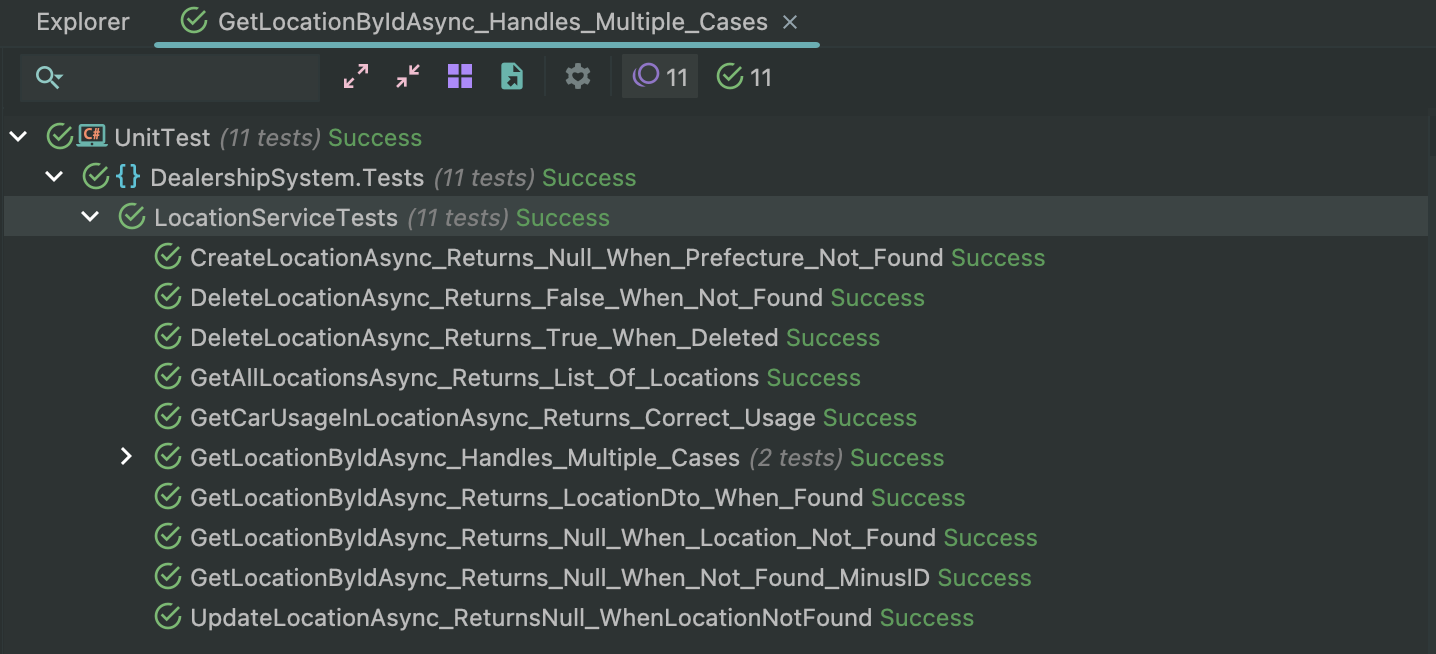
\includegraphics[width=1.0\textwidth]{figures/unittests.png} 
    \caption{A lefutott unit tesztek}
    \label{fig:unittest}
\end{figure}

Az átviteli tesztelésnek az eredményei és kifejtése a WPF, illetve weboldal dokumentációjában történik.

\section{API Végpontok}

\subsection{Autóval kapcsolatos végpontok}

Ez a vezérlő a gépjárművekkel kapcsolatos műveletek kezelését biztosítja, mint például gépjárművek lekérése, létrehozása, frissítése és törlése.

\subsubsection{1. GET /api/cars}

\textbf{Leírás}:  
Ez a végpont lekérdezi az összes gépjárművet a rendszerből.

\textbf{Paraméterek}:  
Nincs.

\textbf{Válasz}:  
\begin{itemize}
    \item \textbf{200 OK}: A gépjárművek listája.
\end{itemize}

\subsubsection{2. GET /api/cars/{id}}

\textbf{Leírás}:  
Ez a végpont egy adott gépjármű adatait kérdezi le az \texttt{id} paraméter alapján.

\textbf{Paraméterek}:  
\begin{itemize}
    \item \texttt{id}: A lekérdezett gépjármű azonosítója (egész szám).
\end{itemize}

\textbf{Válasz}:  
\begin{itemize}
    \item \textbf{200 OK}: A gépjármű adatai.
    \item \textbf{404 Not Found}: Ha nem található a megadott azonosítóval rendelkező gépjármű.
\end{itemize}

\subsubsection{3. POST /api/cars}

\textbf{Leírás}:  
Ez a végpont lehetővé teszi egy új gépjármű létrehozását a rendszerben.

\textbf{Paraméterek}:  
\begin{itemize}
    \item \texttt{CreateCarDTO}: Az új gépjármű adatainak leírása.
\end{itemize}

\textbf{Válasz}:  
\begin{itemize}
    \item \textbf{201 Created}: A gépjármű sikeres létrehozása, a válasz tartalmazza az új gépjármű adatait.
    \item \textbf{400 Bad Request}: Ha a bemeneti adatok érvénytelenek.
\end{itemize}

\subsubsection{4. PUT /api/cars/{id}}

\textbf{Leírás}:  
Ez a végpont frissíti a megadott azonosítóval rendelkező gépjármű adatait.

\textbf{Paraméterek}:  
\begin{itemize}
    \item \texttt{id}: A módosítandó gépjármű azonosítója (egész szám).
    \item \texttt{CreateCarDTO}: Az új gépjármű adatainak leírása.
\end{itemize}

\textbf{Válasz}:  
\begin{itemize}
    \item \textbf{200 OK}: A frissített gépjármű adatai.
    \item \textbf{404 Not Found}: Ha nem található a megadott azonosítóval rendelkező gépjármű.
    \item \textbf{400 Bad Request}: Ha a bemeneti adatok érvénytelenek.
\end{itemize}

\subsubsection{5. DELETE /api/cars/{id}}

\textbf{Leírás}:  
Ez a végpont törli a megadott azonosítóval rendelkező gépjárművet a rendszerből.

\textbf{Paraméterek}:  
\begin{itemize}
    \item \texttt{id}: A törlendő gépjármű azonosítója (egész szám).
\end{itemize}

\textbf{Válasz}:  
\begin{itemize}
    \item \textbf{204 No Content}: A gépjármű sikeres törlése.
    \item \textbf{404 Not Found}: Ha nem található a megadott azonosítóval rendelkező gépjármű.
\end{itemize}

\subsection{Autó gyártóval kapcsolatos végpontok}

Ez a vezérlő az autógyártókkal kapcsolatos műveletek kezelését biztosítja, mint például az autógyártók lekérése, létrehozása, frissítése és törlése.

\subsubsection{1. GET /api/cars/makers}

\textbf{Leírás}:  
Ez a végpont lekérdezi az összes autógyártót a rendszerből.

\textbf{Paraméterek}:  
Nincs.

\textbf{Válasz}:  
\begin{itemize}
    \item \textbf{200 OK}: Az autógyártók listája.
\end{itemize}

\subsubsection{2. GET /api/cars/makers/{id}}

\textbf{Leírás}:  
Ez a végpont egy adott autógyártó adatait kérdezi le az \texttt{id} paraméter alapján.

\textbf{Paraméterek}:  
\begin{itemize}
    \item \texttt{id}: A lekérdezett autógyártó azonosítója (egész szám).
\end{itemize}

\textbf{Válasz}:  
\begin{itemize}
    \item \textbf{200 OK}: Az autógyártó adatai.
    \item \textbf{400 Bad Request}: Ha a megadott azonosítóval nem található autógyártó.
\end{itemize}

\subsubsection{3. POST /api/cars/makers}

\textbf{Leírás}:  
Ez a végpont lehetővé teszi egy új autógyártó létrehozását a rendszerben.

\textbf{Paraméterek}:  
\begin{itemize}
    \item \texttt{CreateCarMakerDTO}: Az új autógyártó adatainak leírása.
\end{itemize}

\textbf{Válasz}:  
\begin{itemize}
    \item \textbf{200 OK}: A sikeres autógyártó létrehozása, a válasz tartalmazza az új autógyártó adatait.
    \item \textbf{400 Bad Request}: Ha a bemeneti adatok érvénytelenek.
    \item \textbf{403 Forbidden}: Ha a műveletet nem lehet végrehajtani.
\end{itemize}

\subsubsection{4. PUT /api/cars/makers}

\textbf{Leírás}:  
Ez a végpont frissíti a megadott autógyártó adatait.

\textbf{Paraméterek}:  
\begin{itemize}
    \item \texttt{UpdateCarMakerDTO}: Az autógyártó frissített adatainak leírása.
\end{itemize}

\textbf{Válasz}:  
\begin{itemize}
    \item \textbf{200 OK}: A frissített autógyártó adatai.
    \item \textbf{400 Bad Request}: Ha a bemeneti adatok érvénytelenek.
\end{itemize}

\subsubsection{5. DELETE /api/cars/makers/{id}}

\textbf{Leírás}:  
Ez a végpont törli a megadott autógyártót a rendszerből.

\textbf{Paraméterek}:  
\begin{itemize}
    \item \texttt{id}: A törlendő autógyártó azonosítója (egész szám).
\end{itemize}

\textbf{Válasz}:  
\begin{itemize}
    \item \textbf{200 OK}: Az autógyártó sikeres törlése.
    \item \textbf{404 Not Found}: Ha nem található a megadott azonosítóval rendelkező autógyártó.
\end{itemize}

\subsection{Autó metaadatokkal kapcsolatos végpontok}

Ez a vezérlő az autókhoz kapcsolódó metaadatok lekérdezését teszi lehetővé, például a karosszériatípusok, váltótípusok, üzemanyagtípusok, hajtáslánc típusok és színek elérését.

\subsubsection{1. GET /api/cars/metadata/bodytypes}

\textbf{Leírás}:  
Lekéri az összes elérhető karosszériatípust.

\textbf{Paraméterek}:  
Nincs.

\textbf{Válasz}:  
\begin{itemize}
    \item \textbf{200 OK}: A karosszériatípusok listája.
\end{itemize}

\subsubsection{2. GET /api/cars/metadata/bodytypes/{id}}

\textbf{Leírás}:  
Lekéri egy adott karosszériatípus adatait.

\textbf{Paraméterek}:  
\begin{itemize}
    \item \texttt{id}: A karosszériatípus azonosítója (egész szám).
\end{itemize}

\textbf{Válasz}:  
\begin{itemize}
    \item \textbf{200 OK}: A kiválasztott karosszériatípus adatai.
    \item \textbf{404 Not Found}: Ha az adott azonosítóval nem található karosszériatípus.
\end{itemize}

\subsubsection{3. GET /api/cars/metadata/transmissionTypes}

\textbf{Leírás}:  
Lekéri az összes elérhető váltótípust.

\textbf{Paraméterek}:  
Nincs.

\textbf{Válasz}:  
\begin{itemize}
    \item \textbf{200 OK}: A váltótípusok listája.
\end{itemize}

\subsubsection{4. GET /api/cars/metadata/transmissionTypes/{id}}

\textbf{Leírás}:  
Lekéri egy adott váltótípus adatait.

\textbf{Paraméterek}:  
\begin{itemize}
    \item \texttt{id}: A váltótípus azonosítója (egész szám).
\end{itemize}

\textbf{Válasz}:  
\begin{itemize}
    \item \textbf{200 OK}: A kiválasztott váltótípus adatai.
    \item \textbf{404 Not Found}: Ha az adott azonosítóval nem található váltótípus.
\end{itemize}

\subsubsection{5. GET /api/cars/metadata/fuelTypes}

\textbf{Leírás}:  
Lekéri az összes elérhető üzemanyagtípust.

\textbf{Paraméterek}:  
Nincs.

\textbf{Válasz}:  
\begin{itemize}
    \item \textbf{200 OK}: Az üzemanyagtípusok listája.
\end{itemize}

\subsubsection{6. GET /api/cars/metadata/fuelTypes/{id}}

\textbf{Leírás}:  
Lekéri egy adott üzemanyagtípus adatait.

\textbf{Paraméterek}:  
\begin{itemize}
    \item \texttt{id}: Az üzemanyagtípus azonosítója (egész szám).
\end{itemize}

\textbf{Válasz}:  
\begin{itemize}
    \item \textbf{200 OK}: A kiválasztott üzemanyagtípus adatai.
    \item \textbf{404 Not Found}: Ha az adott azonosítóval nem található üzemanyagtípus.
\end{itemize}

\subsubsection{7. GET /api/cars/metadata/drivetrainTypes}

\textbf{Leírás}:  
Lekéri az összes elérhető hajtáslánc típust.

\textbf{Paraméterek}:  
Nincs.

\textbf{Válasz}:  
\begin{itemize}
    \item \textbf{200 OK}: A hajtáslánc típusok listája.
\end{itemize}

\subsubsection{8. GET /api/cars/metadata/drivetrainTypes/{id}}

\textbf{Leírás}:  
Lekéri egy adott hajtáslánc típus adatait.

\textbf{Paraméterek}:  
\begin{itemize}
    \item \texttt{id}: A hajtáslánc típus azonosítója (egész szám).
\end{itemize}

\textbf{Válasz}:  
\begin{itemize}
    \item \textbf{200 OK}: A kiválasztott hajtáslánc típus adatai.
    \item \textbf{404 Not Found}: Ha az adott azonosítóval nem található hajtáslánc típus.
\end{itemize}

\subsubsection{9. GET /api/cars/metadata/colors}

\textbf{Leírás}:  
Lekéri az összes elérhető színt.

\textbf{Paraméterek}:  
Nincs.

\textbf{Válasz}:  
\begin{itemize}
    \item \textbf{200 OK}: Az autószínek listája.
\end{itemize}

\subsubsection{10. GET /api/cars/metadata/colors/{id}}

\textbf{Leírás}:  
Lekéri egy adott szín adatait.

\textbf{Paraméterek}:  
\begin{itemize}
    \item \texttt{id}: A szín azonosítója (egész szám).
\end{itemize}

\textbf{Válasz}:  
\begin{itemize}
    \item \textbf{200 OK}: A kiválasztott szín adatai.
    \item \textbf{404 Not Found}: Ha az adott azonosítóval nem található szín.
\end{itemize}

\subsection{Autómodellekkel kapcsolatos végpontok}

Ez a vezérlő az autómodellek kezeléséhez szükséges végpontokat biztosítja, például az autómodellek listázását, keresését, létrehozását, frissítését és törlését.

\subsubsection{1. GET /api/cars/models}

\textbf{Leírás}:  
Lekéri az összes autómodellt.

\textbf{Paraméterek}:  
Nincs.

\textbf{Válasz}:  
\begin{itemize}
    \item \textbf{200 OK}: Az autómodellek listája.
\end{itemize}

\subsubsection{2. POST /api/cars/models}

\textbf{Leírás}:  
Létrehoz egy új autómodellt.

\textbf{Paraméterek}:  
\begin{itemize}
    \item \texttt{CreateCarModelDTO}: Az új autómodell adatai (JSON formátumban).
\end{itemize}

\textbf{Válasz}:  
\begin{itemize}
    \item \textbf{201 Created}: A sikeresen létrehozott autómodell adatai.
    \item \textbf{400 Bad Request}: Hibás kérés esetén, például ha a bemenet érvénytelen.
\end{itemize}

\subsubsection{3. GET /api/cars/models/search}

\textbf{Leírás}:  
Autómodellek keresése megadott szűrési feltételek alapján.

\textbf{Paraméterek}:  
\begin{itemize}
    \item \texttt{makerID} (opcionális) – A gyártó azonosítója.
    \item \texttt{startYear} (opcionális) – A gyártás kezdőéve.
    \item \texttt{endYear} (opcionális) – A gyártás befejező éve.
    \item \texttt{passengerCount} (opcionális) – Az utasok száma.
\end{itemize}

\textbf{Válasz}:  
\begin{itemize}
    \item \textbf{200 OK}: A keresési feltételeknek megfelelő autómodellek listája.
\end{itemize}

\subsubsection{4. PUT /api/cars/models/{id}}

\textbf{Leírás}:  
Frissíti a megadott azonosítójú autómodell adatait.

\textbf{Paraméterek}:  
\begin{itemize}
    \item \texttt{id} – Az autómodell azonosítója.
    \item \texttt{UpdateCarModelDTO} – Az új adatok JSON formátumban.
\end{itemize}

\textbf{Válasz}:  
\begin{itemize}
    \item \textbf{200 OK}: A sikeresen frissített autómodell adatai.
    \item \textbf{400 Bad Request}: Érvénytelen adatok esetén.
    \item \textbf{404 Not Found}: Ha az adott autómodell nem található.
    \item \textbf{500 Internal Server Error}: Ha egyéb hiba történt a frissítés során.
\end{itemize}

\subsubsection{5. DELETE /api/cars/models/{id}}

\textbf{Leírás}:  
Törli a megadott azonosítójú autómodellt.

\textbf{Paraméterek}:  
\begin{itemize}
    \item \texttt{id} – Az autómodell azonosítója.
\end{itemize}

\textbf{Válasz}:  
\begin{itemize}
    \item \textbf{204 No Content}: Sikeres törlés esetén.
    \item \textbf{404 Not Found}: Ha az autómodell nem található.
\end{itemize}

\subsubsection{6. GET /api/cars/models/maker/{makerId}}

\textbf{Leírás}:  
Lekéri egy adott gyártóhoz tartozó autómodelleket.

\textbf{Paraméterek}:  
\begin{itemize}
    \item \texttt{makerId} – Az autógyártó azonosítója.
\end{itemize}

\textbf{Válasz}:  
\begin{itemize}
    \item \textbf{200 OK}: Az adott gyártóhoz tartozó autómodellek listája.
    \item \textbf{404 Not Found}: Ha a gyártóhoz nem tartozik autómodell.
\end{itemize}

\subsection{Alkalmazotti helyszínekkel kapcsolatos végpontok}

Ez a vezérlő az alkalmazotti helyszínek kezeléséhez biztosít végpontokat. Az összes végpont adminisztrátori jogosultságot igényel.

\subsubsection{1. GET /api/employeeLocations}

\textbf{Leírás}:  
Lekéri az összes alkalmazotti helyszínt.

\textbf{Jogosultság}:  
\begin{itemize}
    \item \textbf{Admin} szerepkör szükséges.
\end{itemize}

\textbf{Paraméterek}:  
Nincs.

\textbf{Válasz}:  
\begin{itemize}
    \item \textbf{200 OK}: Az alkalmazotti helyszínek listája.
\end{itemize}

\subsubsection{2. GET /api/employeeLocations/{employeeId}}

\textbf{Leírás}:  
Lekéri egy adott alkalmazott helyszínét.

\textbf{Jogosultság}:  
\begin{itemize}
    \item \textbf{Admin} szerepkör szükséges.
\end{itemize}

\textbf{Paraméterek}:  
\begin{itemize}
    \item \texttt{employeeId} – Az alkalmazott egyedi azonosítója (UUID).
\end{itemize}

\textbf{Válasz}:  
\begin{itemize}
    \item \textbf{200 OK}: Az alkalmazott helyszíne.
    \item \textbf{404 Not Found}: Ha az alkalmazotti helyszín nem található.
\end{itemize}

\subsubsection{3. POST /api/employeeLocations}

\textbf{Leírás}:  
Hozzáad egy új alkalmazotti helyszínt.

\textbf{Jogosultság}:  
\begin{itemize}
    \item \textbf{Admin} szerepkör szükséges.
\end{itemize}

\textbf{Paraméterek}:  
\begin{itemize}
    \item \texttt{EmployeeLocation} – Az új alkalmazotti helyszín adatai (JSON formátumban).
\end{itemize}

\textbf{Válasz}:  
\begin{itemize}
    \item \textbf{201 Created}: A sikeresen létrehozott alkalmazotti helyszín.
    \item \textbf{400 Bad Request}: Ha az adatok érvénytelenek, vagy a helyszín hozzáadása sikertelen.
\end{itemize}

\subsection{Motortípusokkal kapcsolatos végpontok}

Ez a vezérlő az autókhoz tartozó motoradatok kezelésére szolgál.

\subsubsection{1. POST /api/cars/engine}

\textbf{Leírás}:  
Új motortípus létrehozása egy adott autómodellhez.

\textbf{Paraméterek}:  
\begin{itemize}
    \item \texttt{CreateEngineDTO} – A motor adatai (JSON formátumban):
    \begin{itemize}
        \item \texttt{ModelID} – Az autómodell azonosítója.
        \item \texttt{EngineSize} – A motor mérete.
        \item \texttt{FuelType} – Az üzemanyagtípus.
    \end{itemize}
\end{itemize}

\textbf{Válasz}:  
\begin{itemize}
    \item \textbf{200 OK}: A sikeresen létrehozott motoradatok.
    \item \textbf{400 Bad Request}: Ha az adatok érvénytelenek.
\end{itemize}

\subsubsection{2. GET /api/cars/engine/model/\{modelId\}}

\textbf{Leírás}:  
Lekéri egy adott autómodellhez tartozó motortípusokat.

\textbf{Paraméterek}:  
\begin{itemize}
    \item \texttt{modelId} – Az autómodell egyedi azonosítója.
\end{itemize}

\textbf{Válasz}:  
\begin{itemize}
    \item \textbf{200 OK}: Az adott autómodellhez tartozó motorok listája.
    \item \textbf{404 Not Found}: Ha nincs elérhető motortípus a modellhez.
\end{itemize}

\subsubsection{3. PUT /api/cars/engine/update}

\textbf{Leírás}:  
Egy meglévő motoradat módosítása.

\textbf{Paraméterek}:  
\begin{itemize}
    \item \texttt{UpdateEngineDTO} – A módosított motoradatok (JSON formátumban):
    \begin{itemize}
        \item \texttt{ID} – A motor azonosítója.
        \item \texttt{NewEngineSize} – Az új motor mérete.
        \item \texttt{FuelTypeID} – Az új üzemanyagtípus azonosítója.
    \end{itemize}
\end{itemize}

\textbf{Válasz}:  
\begin{itemize}
    \item \textbf{200 OK}: A sikeresen módosított motoradatok.
    \item \textbf{400 Bad Request}: Ha az adatok érvénytelenek.
    \item \textbf{404 Not Found}: Ha a motor nem található.
\end{itemize}

\subsubsection{4. DELETE /api/cars/engine/\{engineId\}}

\textbf{Leírás}:  
Egy adott motoradat törlése.

\textbf{Paraméterek}:  
\begin{itemize}
    \item \texttt{engineId} – A törlendő motor egyedi azonosítója.
\end{itemize}

\textbf{Válasz}:  
\begin{itemize}
    \item \textbf{200 OK}: A sikeres törlés.
    \item \textbf{404 Not Found}: Ha a motor nem található.
\end{itemize}

\subsection{Képkezeléssel kapcsolatos végpontok}

Ez a vezérlő az autókhoz tartozó képek feltöltésére és lekérdezésére szolgál.

\subsubsection{1. POST /api/images/upload}

\textbf{Leírás}:  
Egy új kép feltöltése egy adott autóhoz.

\textbf{Paraméterek}:  
\begin{itemize}
    \item \texttt{ImageUploadDto} – A feltöltendő kép adatai (multipart form-data):
    \begin{itemize}
        \item \texttt{ImageFile} – A feltöltendő kép fájlja.
        \item \texttt{CarID} – Az autó azonosítója, amelyhez a kép tartozik.
    \end{itemize}
\end{itemize}

\textbf{Válasz}:  
\begin{itemize}
    \item \textbf{200 OK}: Sikeres feltöltés esetén a visszakapott kép URL-je.
    \item \textbf{400 Bad Request}: Ha a feltöltés sikertelen.
\end{itemize}

\subsubsection{2. GET /api/images/car/\{carId\}}

\textbf{Leírás}:  
Lekéri egy adott autóhoz tartozó képeket.

\textbf{Paraméterek}:  
\begin{itemize}
    \item \texttt{carId} – Az autó egyedi azonosítója.
\end{itemize}

\textbf{Válasz}:  
\begin{itemize}
    \item \textbf{200 OK}: Az adott autóhoz tartozó képek listája.
    \item \textbf{404 Not Found}: Ha az autóhoz nem tartoznak képek.
\end{itemize}

\subsection{Telephelyekkel kapcsolatos végpontok}

Ez a vezérlő a telephelyek kezelésére szolgál.

\subsubsection{1. GET /api/locations}

\textbf{Leírás}:  
Lekéri az összes telephelyet.

\textbf{Válasz}:  
\begin{itemize}
    \item \textbf{200 OK}: A telephelyek listája.
    \item \textbf{204 No Content}: Ha nincs elérhető telephely.
\end{itemize}

\subsubsection{2. GET /api/locations/prefectures}

\textbf{Leírás}:  
Lekéri az összes prefektúrát.

\textbf{Válasz}:  
\begin{itemize}
    \item \textbf{200 OK}: A prefektúrák listája.
\end{itemize}

\subsubsection{3. GET /api/locations/\{id\}}

\textbf{Leírás}:  
Lekér egy telephelyet azonosító alapján.

\textbf{Paraméterek}:  
\begin{itemize}
    \item \texttt{id} – A telephely azonosítója.
\end{itemize}

\textbf{Válasz}:  
\begin{itemize}
    \item \textbf{200 OK}: A telephely adatai.
    \item \textbf{404 Not Found}: Ha a telephely nem található.
\end{itemize}

\subsubsection{4. POST /api/locations}

\textbf{Leírás}:  
Új telephely létrehozása. Csak adminisztrátorok számára elérhető.

\textbf{Fejlécek}:  
\begin{itemize}
    \item \texttt{Authorization: Bearer <token>} – Adminisztrátori jogosultság szükséges.
\end{itemize}

\textbf{Törzs}:  
\begin{itemize}
    \item \texttt{LocationDto} – A létrehozandó telephely adatai.
\end{itemize}

\textbf{Válasz}:  
\begin{itemize}
    \item \textbf{200 OK}: A létrehozott telephely.
    \item \textbf{422 Unprocessable Entity}: Ha a létrehozás sikertelen.
\end{itemize}

\subsubsection{5. PUT /api/locations/update}

\textbf{Leírás}:  
Telephely adatainak frissítése. Csak adminisztrátorok számára elérhető.

\textbf{Fejlécek}:  
\begin{itemize}
    \item \texttt{Authorization: Bearer <token>} – Adminisztrátori jogosultság szükséges.
\end{itemize}

\textbf{Törzs}:  
\begin{itemize}
    \item \texttt{LocationDto} – A frissítendő telephely adatai.
\end{itemize}

\textbf{Válasz}:  
\begin{itemize}
    \item \textbf{200 OK}: A frissített telephely.
    \item \textbf{400 Bad Request}: Ha a bemeneti adatok érvénytelenek.
    \item \textbf{404 Not Found}: Ha a telephely nem található.
    \item \textbf{500 Internal Server Error}: Ha belső hiba történik.
\end{itemize}

\subsubsection{6. DELETE /api/locations/\{locationId\}}

\textbf{Leírás}:  
Egy telephely törlése. Csak adminisztrátorok számára elérhető.

\textbf{Fejlécek}:  
\begin{itemize}
    \item \texttt{Authorization: Bearer <token>} – Adminisztrátori jogosultság szükséges.
\end{itemize}

\textbf{Paraméterek}:  
\begin{itemize}
    \item \texttt{locationId} – A törlendő telephely azonosítója.
\end{itemize}

\textbf{Válasz}:  
\begin{itemize}
    \item \textbf{200 OK}: Sikeres törlés.
    \item \textbf{204 No Content}: Ha a telephely nem található.
    \item \textbf{500 Internal Server Error}: Ha belső hiba történt.
\end{itemize}

\subsubsection{7. GET /api/locations/\{locationId\}/car-usage}

\textbf{Leírás}:  
Lekéri egy telephely autóhasználati adatait.

\textbf{Paraméterek}:  
\begin{itemize}
    \item \texttt{locationId} – A telephely azonosítója.
\end{itemize}

\textbf{Válasz}:  
\begin{itemize}
    \item \textbf{200 OK}: Az aktuális és maximális kapacitás adatai.
    \item \textbf{404 Not Found}: Ha a telephely nem található.
\end{itemize}

\subsection{Üzenetekkel kapcsolatos végpontok}

Ez a vezérlő az üzenetek lekérdezésére és törlésére szolgál.

\subsubsection{1. GET /api/messages/\{userId\}}

\textbf{Leírás}:  
Lekéri egy adott felhasználóhoz tartozó üzeneteket.

\textbf{Paraméterek}:  
\begin{itemize}
    \item \texttt{userId} – A felhasználó azonosítója (GUID formátumban).
\end{itemize}

\textbf{Válasz}:  
\begin{itemize}
    \item \textbf{200 OK}: Az üzenetek listája.
    \item \textbf{401 Unauthorized}: Ha a felhasználó nem jogosult az üzenetek megtekintésére.
\end{itemize}

\subsubsection{2. DELETE /api/messages/\{messageId\}}

\textbf{Leírás}:  
Törli az adott azonosítójú üzenetet.

\textbf{Paraméterek}:  
\begin{itemize}
    \item \texttt{messageId} – A törlendő üzenet azonosítója.
\end{itemize}

\textbf{Válasz}:  
\begin{itemize}
    \item \textbf{204 No Content}: Sikeres törlés.
    \item \textbf{404 Not Found}: Ha az üzenet nem található.
    \item \textbf{401 Unauthorized}: Ha a felhasználó nem jogosult az üzenet törlésére.
\end{itemize}


\subsection{Foglalásokkal kapcsolatos végpontok}

Ez a vezérlő a felhasználók foglalásainak kezelésére szolgál.

\subsubsection{1. GET /api/reservations}

\textbf{Leírás}:  
Lekéri a bejelentkezett felhasználó összes foglalását.

\textbf{Válasz}:  
\begin{itemize}
    \item \textbf{200 OK}: A felhasználó foglalásainak listája.
    \item \textbf{401 Unauthorized}: Ha a felhasználó nincs bejelentkezve.
\end{itemize}

\subsubsection{2. GET /api/reservations/\{id\}}

\textbf{Leírás}:  
Lekéri az adott foglalás adatait.

\textbf{Paraméterek}:  
\begin{itemize}
    \item \texttt{id} – A foglalás azonosítója.
\end{itemize}

\textbf{Válasz}:  
\begin{itemize}
    \item \textbf{200 OK}: A foglalás adatai.
    \item \textbf{401 Unauthorized}: Ha a felhasználó nincs bejelentkezve.
    \item \textbf{404 Not Found}: Ha a foglalás nem található.
\end{itemize}

\subsubsection{3. POST /api/reservations}

\textbf{Leírás}:  
Új foglalást hoz létre a bejelentkezett felhasználó számára.

\textbf{Törzs (Body)}:  
\texttt{CreateReservationDTO} objektumot vár.

\textbf{Válasz}:  
\begin{itemize}
    \item \textbf{201 Created}: A létrehozott foglalás adatai.
    \item \textbf{401 Unauthorized}: Ha a felhasználó nincs bejelentkezve.
    \item \textbf{403 Forbidden}: Ha a felhasználónak nincs jogosultsága a foglalás létrehozásához.
\end{itemize}

\subsubsection{4. PUT /api/reservations/\{id\}}

\textbf{Leírás}:  
Frissíti az adott foglalás adatait.

\textbf{Paraméterek}:  
\begin{itemize}
    \item \texttt{id} – A frissítendő foglalás azonosítója.
\end{itemize}

\textbf{Törzs (Body)}:  
\texttt{UpdateReservationDTO} objektumot vár.

\textbf{Válasz}:  
\begin{itemize}
    \item \textbf{200 OK}: A frissített foglalás adatai.
    \item \textbf{401 Unauthorized}: Ha a felhasználó nincs bejelentkezve.
    \item \textbf{404 Not Found}: Ha a foglalás nem található.
\end{itemize}

\subsubsection{5. DELETE /api/reservations/\{id\}}

\textbf{Leírás}:  
Törli az adott foglalást.

\textbf{Paraméterek}:  
\begin{itemize}
    \item \texttt{id} – A törlendő foglalás azonosítója.
\end{itemize}

\textbf{Válasz}:  
\begin{itemize}
    \item \textbf{204 No Content}: Sikeres törlés.
    \item \textbf{401 Unauthorized}: Ha a felhasználó nincs bejelentkezve.
    \item \textbf{404 Not Found}: Ha a foglalás nem található.
\end{itemize}


\subsection{Mentett autókkal kapcsolatos végpontok}

Ez a vezérlő a felhasználók által mentett autók kezelésére szolgál.

\subsubsection{1. GET /api/savedcars/\{userId\}}

\textbf{Leírás}:  
Lekéri a megadott felhasználó által mentett autók azonosítóit.

\textbf{Paraméterek}:  
\begin{itemize}
    \item \texttt{userId} – A felhasználó azonosítója (GUID formátumban).
\end{itemize}

\textbf{Válasz}:  
\begin{itemize}
    \item \textbf{200 OK}: A felhasználó által mentett autók azonosítóinak listája.
    \item \textbf{401 Unauthorized}: Ha a felhasználó nem jogosult az adatok lekérésére.
    \item \textbf{500 Internal Server Error}: Ha váratlan hiba történt.
\end{itemize}

\subsubsection{2. POST /api/savedcars/\{userId\}/save}

\textbf{Leírás}:  
Ment egy autót a felhasználó számára.

\textbf{Paraméterek}:  
\begin{itemize}
    \item \texttt{userId} – A felhasználó azonosítója (GUID formátumban).
\end{itemize}

\textbf{Törzs (Body)}:  
\begin{itemize}
    \item Egyetlen \texttt{carId} érték (az autó azonosítója, egész szám).
\end{itemize}

\textbf{Válasz}:  
\begin{itemize}
    \item \textbf{204 No Content}: Sikeres mentés.
    \item \textbf{401 Unauthorized}: Ha a felhasználó nem jogosult az autó mentésére.
    \item \textbf{500 Internal Server Error}: Ha váratlan hiba történt.
\end{itemize}

\subsubsection{3. DELETE /api/savedcars/\{userId\}/remove/\{carId\}}

\textbf{Leírás}:  
Eltávolít egy mentett autót a felhasználó listájából.

\textbf{Paraméterek}:  
\begin{itemize}
    \item \texttt{userId} – A felhasználó azonosítója (GUID formátumban).
    \item \texttt{carId} – Az eltávolítandó autó azonosítója (egész szám).
\end{itemize}

\textbf{Válasz}:  
\begin{itemize}
    \item \textbf{204 No Content}: Sikeres törlés.
    \item \textbf{401 Unauthorized}: Ha a felhasználó nem jogosult a törlésre.
    \item \textbf{500 Internal Server Error}: Ha váratlan hiba történt.
\end{itemize}


\subsection{Felhasználókkal kapcsolatos végpontok}

Ez a vezérlő a felhasználók kezelésére szolgál.

\subsubsection{1. POST /api/users/register}

\textbf{Leírás}:  
Új felhasználó regisztrálása.

\textbf{Törzs (Body)}:  
\begin{itemize}
    \item Felhasználói adatok, mint email cím, jelszó, név, telefonszám és preferált nyelv.
\end{itemize}

\textbf{Válasz}:  
\begin{itemize}
    \item \textbf{200 OK}: A felhasználó sikeresen regisztrálva lett.
    \item \textbf{400 Bad Request}: Ha az email cím már foglalt, vagy ha érvénytelen adatokat adtak meg.
\end{itemize}

\subsubsection{2. POST /api/users/login}

\textbf{Leírás}:  
Felhasználó bejelentkezése.

\textbf{Törzs (Body)}:  
\begin{itemize}
    \item Felhasználói email cím és jelszó.
\end{itemize}

\textbf{Válasz}:  
\begin{itemize}
    \item \textbf{200 OK}: A felhasználó sikeresen bejelentkezett.
    \item \textbf{401 Unauthorized}: Ha a felhasználói adatok helytelenek.
\end{itemize}

\subsubsection{3. PUT /api/users/\{userId\}/update}

\textbf{Leírás}:  
A felhasználó adatainak frissítése.

\textbf{Paraméterek}:  
\begin{itemize}
    \item \texttt{userId} – A frissíteni kívánt felhasználó azonosítója.
\end{itemize}

\textbf{Törzs (Body)}:  
\begin{itemize}
    \item Frissített felhasználói adatok: név, telefonszám, preferált nyelv.
\end{itemize}

\textbf{Válasz}:  
\begin{itemize}
    \item \textbf{200 OK}: A felhasználói adatok sikeresen frissítve lettek.
    \item \textbf{400 Bad Request}: Ha érvénytelen adatokat adtak meg.
    \item \textbf{401 Unauthorized}: Ha a felhasználó nem jogosult a frissítésre.
\end{itemize}

\subsubsection{4. DELETE /api/users/\{userId\}}

\textbf{Leírás}:  
Felhasználó törlése.

\textbf{Paraméterek}:  
\begin{itemize}
    \item \texttt{userId} – A törölni kívánt felhasználó azonosítója.
\end{itemize}

\textbf{Válasz}:  
\begin{itemize}
    \item \textbf{204 No Content}: A felhasználó sikeresen törölve lett.
    \item \textbf{401 Unauthorized}: Ha a felhasználó nem jogosult a törléshez.
    \item \textbf{500 Internal Server Error}: Ha váratlan hiba történt.
\end{itemize}



\chapter{WPF dokumentációja}

\section{Bevezetés}
Ez a rész a WPF kliens alkalmazásának telepítését, konfigurációját és működését mutatja be. Az alkalmazás egy backend szerverhez csatlakozik HTTP API-n keresztül.

\section{Telepítés és Konfiguráció}
\subsection{Forráskód és Fordítás}
A projekt Visual Studio segítségével fordítható. A forráskódban található \texttt{HttpClientService.cs} fájlban módosítani kell a backend szerver címét:

\begin{verbatim}
client = new HttpClient(tokenRefreshHandler)
{
BaseAddress = new Uri("https://192.168.1.100:7268")
};
\end{verbatim}

Ezt a megfelelő IP-címre vagy domain névre kell cserélni a helyes működés érdekében.

\subsection{Függőségek}
Az alkalmazás a következő NuGet csomagokat használja:
\begin{itemize}
\item Newtonsoft.Json
\item System.Net.Http
\end{itemize}

\section{Felépítés és Ablakok}
Az alkalmazás több ablakból és oldalból áll:

\subsection{Ablakok (Windows)}
\begin{itemize}
\item \texttt{LoginWindow.xaml}
\item \texttt{AddCarWindow.xaml}
\item \texttt{EditCarWindow.xaml}
\item \texttt{EditCarModelWindow.xaml}
\item \texttt{EditLocationWindow.xaml}
\item \texttt{AddLocationWindow.xaml}
\item \texttt{CreateNewCarModelWindow.xaml}
\item \texttt{EditUserWindow.xaml}
\item \texttt{EditCarMakerWindow.xaml}
\item \texttt{AddUserWindow.xaml}
\item \texttt{AddEngineWindow.xaml}
\end{itemize}

\subsection{Oldalak (Pages)}
\begin{itemize}
\item \texttt{CarModelPage.xaml}
\item \texttt{CarsPage.xaml}
\item \texttt{UserPage.xaml}
\item \texttt{CarMakersPage.xaml}
\item \texttt{LocationsPage.xaml}
\end{itemize}

\section{Első indítás és bejelentkezés}
\begin{itemize}
    \item Indítsd el a PremiumCars alkalmazást.
    \item Ha a szerver (API) nem fut, a kliens nem fog tudni kapcsolódni, és a következő hiba jelenhet meg: \texttt{Could not connect to server}.
    \item Bejelentkezés admin jogosultságú felhasználóval (felhasználónév/jelszó). Hibás adatok esetén: \texttt{Unauthorized} vagy \texttt{Invalid credentials}.
\end{itemize}

\section{Autók kezelése}

\subsection{Új autó hozzáadása}
\begin{itemize}
    \item Kérés: \texttt{POST /api/cars}
    \item Kötelező adatok:
    \begin{itemize}
        \item \textbf{brand}: autómárka (pl. Toyota, BMW).
        \item \textbf{model}: a kiválasztott márkához tartozó modell.
        \item \textbf{engineSize}: motoradat (köbcenti, üzemanyag).
        \item \textbf{bodyType}: karosszériatípus (SUV, Sedan, Hatchback stb.).
        \item \textbf{locationId}: a telephely, ahol az autó elérhető.
        \item \textbf{price}, \textbf{licensePlateNumber}, \textbf{MOTExpiry}, \textbf{VINNum}: az autó egyéb adatai.
    \end{itemize}
    \item Képfeltöltés: fájlok (jpg, png), max. 5-10 MB/kép.
    \item Válaszok:
    \begin{itemize}
        \item Siker: \texttt{200 OK} – „Car added successfully!”
        \item Hiányzó mező: \texttt{400 Bad Request} – hibajelzés a hiányzó mező nevével.
    \end{itemize}
\end{itemize}

\subsection{Meglévő autó módosítása}
\begin{itemize}
    \item Kérés: \texttt{PUT /api/cars/\{id\}}
    \item Adatmódosítások:
    \begin{itemize}
        \item Ár (\textbf{price}) frissítése.
        \item Kilométeróra állása (\textbf{mileage}) módosítása.
        \item Rendszám (\textbf{licensePlateNumber}) javítása.
        \item Képek cseréje (backend támogatás esetén).
    \end{itemize}
    \item Válaszok:
    \begin{itemize}
        \item Siker: \texttt{200 OK} – „Autó adatai frissültek!”
        \item Nem létező ID: \texttt{404 Not Found}.
    \end{itemize}
\end{itemize}

\section{Helyszínek kezelése}
\subsection{Új telephely hozzáadása}
\begin{itemize}
    \item Kérés: \texttt{POST /api/locations}
    \item Kötelező adatok:
    \begin{itemize}
        \item \textbf{locationName}, \textbf{address} (irányítószám, város, utca, prefektúra).
        \item \textbf{maxCapacity}: maximális kapacitás.
        \item \textbf{phoneNumber}: telefonszám.
    \end{itemize}
    \item Duplikáció ellenőrzése: ha az adott cím már létezik, \texttt{400 Bad Request}.
\end{itemize}

\subsection{Telephely módosítása}
\begin{itemize}
    \item Kérés: \texttt{PUT /api/locations/\{id\}}
    \item Az adatok előtöltve jelennek meg szerkesztéskor.
\end{itemize}

\section{Motoradatok, Márkák, Modellek szerkesztése}
\begin{itemize}
    \item \texttt{POST /api/cars/engine} – új motoradatok felvitele (\textbf{engineSize}, \textbf{fuelType}).
    \item \texttt{PUT /api/cars/makers} – márkák szerkesztése (\textbf{brandEnglish}, \textbf{brandJapanese}).
    \item \texttt{PUT /api/cars/models/\{id\}} – modellek módosítása (\textbf{modelNameEnglish}, \textbf{manufacturingStartYear}, \textbf{passengerCount}).
\end{itemize}

\section{Gyakori hibák és megoldások}
\subsection{Szerverelérési problémák}
\begin{itemize}
    \item \texttt{Could not connect to server} vagy \texttt{404 Not Found} esetén:
    \begin{itemize}
        \item Ellenőrizd, hogy a szerver fut-e.
        \item Győződj meg róla, hogy a hálózati kapcsolat él.
        \item Tűzfal beállítások ellenőrzése.
    \end{itemize}
\end{itemize}

\subsection{Érvénytelen beviteli adatok}
\begin{itemize}
    \item \textbf{Mileage}: csak számokat fogad el. Hiba esetén: \texttt{Invalid integer format}.
    \item \textbf{VINNum}: max. 17 karakter lehet. Hosszabb adatnál: \texttt{400 Bad Request}.
    \item \textbf{MOTExpiry}: elvárt formátum: \texttt{YYYY-MM-DD}.
\end{itemize}

\section{Tesztkörnyezet}
Az alkalmazás tesztelése az alábbi környezetben történt:
\begin{itemize}
    \item Hardver: Apple M1 (ARM architektúra)
    \item Operációs rendszer: Windows 11 ARM, japán nyelvi beállításokkal
    \item Képernyőfelbontás: 1920x1080
    \item Böngésző: Google Chrome (legújabb verzió)
\end{itemize}

Megjegyzés: Noha bizonyos mezők japán nyelvű bemenethez specializáltak, ezek validálása nem történik meg, mivel az túlzottan korlátozó lenne, és nehezítené az egynyelvű tesztelést. Ha egy mező japán karaktereket kér, akkor a helyes eljárás a latin betűs bevitel vagy adott esetben a mező figyelmen kívül hagyása (pl. név Kanji mező, amelyet magyar és angol nyelvű felhasználók jellemzően nem használnak).

\section{Teszt Esetek}

\subsection{Üres modell név esetén hibaüzenet}
Ha a modell neve üres, a rendszer hibát dob: \texttt{Modell neve nem lehet üres}.

\begin{figure}[H]
    \centering
    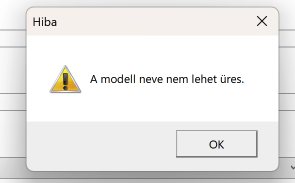
\includegraphics[width=0.8\textwidth]{figures/empty_model_name_error.png}
    \caption{Hibaüzenet üres modellnév esetén}
    \label{fig:empty_model}
\end{figure}

\subsection{Üres helyszín név esetén hibaüzenet}
Ha a helyszín neve nincs kitöltve, a rendszer az alábbi hibát dobja: \texttt{A helyszín neve kötelező}.

\begin{figure}[H]
    \centering
    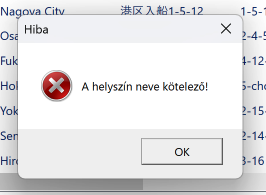
\includegraphics[width=0.8\textwidth]{figures/location_name_empty_error.png}
    \caption{Hibaüzenet üres helyszínnév esetén}
    \label{fig:empty_location}
\end{figure}

\subsection{Nincs kiválasztva prefektúra}
Ha a felhasználó nem választ ki prefektúrát, a következő hibaüzenet jelenik meg: \texttt{Prefektúra kiválasztása kötelező}.

\begin{figure}[H]
    \centering
    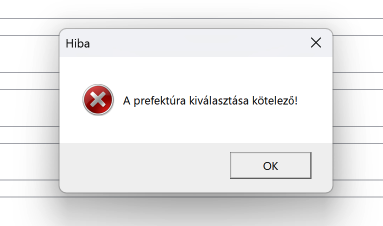
\includegraphics[width=0.8\textwidth]{figures/prefecture_not_selected_error.png}
    \caption{Hibaüzenet hiányzó prefektúra esetén}
    \label{fig:missing_prefecture}
\end{figure}

\subsection{Üres irányítószám}
Ha az irányítószám nincs kitöltve, a rendszer az alábbi hibaüzenetet jeleníti meg: \texttt{Az irányítószám kitöltése kötelező}.

\begin{figure}[H]
    \centering
    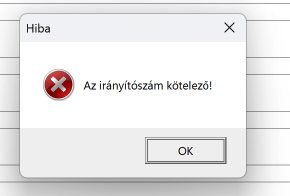
\includegraphics[width=0.8\textwidth]{figures/postal_code_not_input_error.png}
    \caption{Hibaüzenet üres irányítószám esetén}
    \label{fig:empty_postal}
\end{figure}

\subsection{Üres utcanév esetén hibaüzenet}
Ha az utca neve nincs kitöltve, a következő hibaüzenet jelenik meg: \texttt{Az utca neve kötelező}.

\begin{figure}[H]
    \centering
    
\includegraphics[width=0.8\textwidth]{figures/street_name_not_included_error.png}
    \caption{Hibaüzenet üres utcanév esetén}
    \label{fig:empty_street}
\end{figure}

\subsection{Érvénytelen maximális kapacitás}
Ha a maximális kapacitás nem pozitív szám, a rendszer a következő hibát dobja: \texttt{A maximális kapacitás érvényes pozitív szám kell hogy legyen}.

\begin{figure}[H]
    \centering
    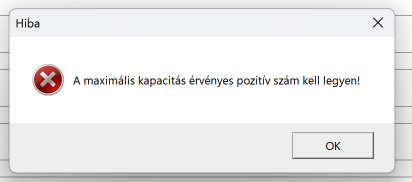
\includegraphics[width=0.8\textwidth]{figures/capacity_input_error.png}
    \caption{Hibaüzenet érvénytelen kapacitás esetén}
    \label{fig:invalid_capacity}
\end{figure}

\subsection{Új felhasználó létrehozása név nélkül}
Ha az új felhasználó neve nincs megadva, a rendszer az alábbi hibát dobja: \texttt{A név megadása kötelező}.

\begin{figure}[H]
    \centering
    
\includegraphics[width=0.8\textwidth]{figures/name_not_input_error.png}
    \caption{Hibaüzenet üres felhasználónév esetén}
    \label{fig:missing_user_name}
\end{figure}

\section{További fejlesztési tervek}
\begin{itemize}
    \item \textbf{Statisztikák}: autók száma telephelyenként, átlagos értékesítési idő, legnépszerűbb márkák.
    \item \textbf{Felhasználókezelés}: admin jogok kezelése, moderátorok hozzáadása, fiókok felfüggesztése.
    \item \textbf{Riportok és kimutatások}: PDF export, grafikonok, statisztika.
\end{itemize}


\section{Backend Kommunikáció}
Az alkalmazás a backend API-val való kommunikációhoz a \texttt{HttpClientService} osztályt használja, amely biztosítja az authentikációt és a token frissítést.

\section{Token Frissítés és HTTP Kérések Kezelése}
A \texttt{WPF} kliens alkalmazás a \texttt{HttpClientService} és a \texttt{TokenRefreshHttpHandler} osztályokat használja a backend API-val való kommunikáció során. A következő szakasz részletesebben bemutatja ezek működését és az egyes lépések logikáját.

\subsection{TokenRefreshHttpHandler – Kérések és Token Frissítés Kezelése}
A \texttt{TokenRefreshHttpHandler} egy egyedi \texttt{DelegatingHandler}, amely figyeli a kérések válaszát, és ha az \texttt{401 Unauthorized} státuszkódot kap, automatikusan megpróbálja frissíteni a hozzáférési tokent.

\subsubsection{Folyamat:}
\begin{enumerate}
    \item \textbf{Elsődleges kérés küldése:}  
    Az osztály először naplózza a küldött kérést (\texttt{Debug.WriteLine} segítségével).  
    Továbbítja a kérést az alatta lévő \texttt{HttpMessageHandler} példánynak.  
    Naplózza a kapott választ (\texttt{Debug.WriteLine}).
    
    \item \textbf{401 Unauthorized válasz kezelése:}  
    Ha a szerver \texttt{401 Unauthorized} válasszal reagál, az azt jelenti, hogy a hozzáférési token lejárt.  
    Naplózza az eseményt: \texttt{"Token expired, attempting to refresh..."}  
    Meghívja a \texttt{HttpClientService.RefreshTokenIfNeeded()} metódust.
    
    \item \textbf{Token frissítés és újrapróbálkozás:}  
    Ha a token frissítés sikeres:  
    \begin{itemize}
        \item Lekéri az új hozzáférési tokent a \texttt{HttpClientService.GetAccessToken()} metódussal.
        \item Frissíti a kérés fejlécében az \texttt{Authorization} mezőt az új tokennel.
        \item Ismét elküldi az eredeti kérést.
    \end{itemize}
    Ha a frissítés sikertelen, a válasz változatlanul visszatér.
\end{enumerate}

\subsubsection{Példa:}
A következő kódrészlet mutatja, hogyan történik a token frissítés és újrapróbálkozás a \texttt{401 Unauthorized} státuszkód esetén:

\begin{lstlisting}[language=csharp]
if (response.StatusCode == HttpStatusCode.Unauthorized)
{
    Debug.WriteLine("Token expired, attempting to refresh...");

    bool refreshSuccess = await HttpClientService.RefreshTokenIfNeeded();

    if (refreshSuccess)
    {
        var newAccessToken = HttpClientService.GetAccessToken();
        if (!string.IsNullOrEmpty(newAccessToken))
        {
            Debug.WriteLine("Access token refreshed, retrying request with new token.");
            request.Headers.Authorization = new System.Net.Http.Headers.AuthenticationHeaderValue("Bearer", newAccessToken);
            response = await base.SendAsync(request, cancellationToken);
        }
        else
        {
            Debug.WriteLine("Failed to get new access token.");
        }
    }
    else
    {
        Debug.WriteLine("Token refresh failed.");
    }
}
\end{lstlisting}

\subsection{HttpClientService – HTTP Kliens Kezelése}
A \texttt{HttpClientService} egy statikus osztály, amely az alábbi funkciókat látja el:
\begin{itemize}
    \item \textbf{HTTP kliens inicializálása} a megfelelő \texttt{HttpMessageHandler} lánccal.
    \item \textbf{Süti kezelés (\texttt{CookieContainer})} az autentikációs adatok tárolására.
    \item \textbf{Token frissítési mechanizmus} a \texttt{RefreshTokenIfNeeded()} metódussal.
\end{itemize}

\subsubsection{Fontos változók és objektumok:}
\begin{lstlisting}[language=csharp]
private static readonly CookieContainer cookieContainer;
private static readonly HttpClientHandler handler;
private static readonly HttpClient client;
\end{lstlisting}

\subsubsection{Token frissítés folyamata:}
\begin{enumerate}
    \item \textbf{Refresh token kinyerése a sütikből.}
    \item \textbf{Token frissítési kérelem küldése a szerver \texttt{/api/users/refresh} végpontjára.}
    \item \textbf{Ha a válasz sikeres (\texttt{200 OK}), az új tokenek mentése sütiként.}
    \item \textbf{Ha a frissítés sikertelen, az eredeti válasz visszaadása.}
\end{enumerate}

\subsubsection{Kód:}
\begin{lstlisting}[language=csharp]
public static async Task<bool> RefreshTokenIfNeeded()
{
    var cookies = cookieContainer.GetCookies(client.BaseAddress);
    var refreshToken = cookies["RefreshToken"]?.Value;

    if (refreshToken != null)
    {
        var content = new StringContent($"\"{refreshToken}\"", Encoding.UTF8, "application/json");
        HttpResponseMessage response = await client.PostAsync("/api/users/refresh", content);

        if (response.IsSuccessStatusCode)
        {
            var responseContent = await response.Content.ReadAsStringAsync();
            var newTokens = JsonSerializer.Deserialize<TokenResponseDTO>(responseContent, new JsonSerializerOptions { PropertyNameCaseInsensitive = true });

            if (newTokens?.AccessToken != null)
            {
                AddCookie("AccessToken", newTokens.AccessToken, client.BaseAddress.ToString());
                AddCookie("RefreshToken", newTokens.RefreshToken, client.BaseAddress.ToString());
                return true;
            }
        }
    }

    return false;
}
\end{lstlisting}

\section{Összegzés}
Az alkalmazás a \texttt{TokenRefreshHttpHandler} és a \texttt{HttpClientService} osztályok segítségével biztosítja, hogy az autentikációs tokenek automatikusan frissüljenek, ha azok lejárnak, anélkül hogy a felhasználónak újra be kellene jelentkeznie. A \texttt{TokenRefreshHttpHandler} a HTTP kérések kezelésére szolgál, és ha \texttt{401 Unauthorized} válasz érkezik, megpróbálja frissíteni a hozzáférési tokent és újraküldi a kérést. A \texttt{HttpClientService} felelős az autentikációs sütik tárolásáért és a tokenek frissítéséért. A kód és a példák bemutatják, hogyan történik a tokenek kezelése és a kérések újraküldése a frissített tokenekkel.

\chapter{Frontend}
\section{Telepítési Útmutató}

Ez az útmutató bemutatja, hogyan telepítheted és futtathatod a React alapú alkalmazást a fejlesztői környezetedben.

\section{Előfeltételek}

Mielőtt nekiállnál a telepítésnek, győződj meg róla, hogy az alábbi szoftverek telepítve vannak a gépeden:

\begin{itemize}
    \item \textbf{Node.js}: A React alkalmazás futtatásához szükséges. A Node.js letöltéséhez és telepítéséhez látogass el a \url{https://nodejs.org/} weboldalra.
    \item \textbf{npm (Node Package Manager)}: Az npm alapértelmezés szerint telepítve van a Node.js-sel együtt.
\end{itemize}

A telepítés után ellenőrizheted, hogy a Node.js és az npm helyesen telepítve van a következő parancsok futtatásával:

\begin{verbatim}
node -v
npm -v
\end{verbatim}

\section{Alkalmazás Telepítése}

Miután a projektet klónoztad, kövesd az alábbi lépéseket:

\subsection{Navigálj a frontend könyvtárba}

A projekt mappájában lépj a frontend könyvtárba:

\begin{verbatim}
cd frontend
\end{verbatim}

\subsection{Függőségek telepítése}

A projekt összes szükséges csomagját és függőségét az npm telepíti a következő parancs futtatásával:

\begin{verbatim}
npm install
\end{verbatim}

Ez letölti a projektben meghatározott összes függőséget a \texttt{node\_modules} mappába.

\subsection{IP cím módosítása (ha szükséges)}

A backend szerver IP-címét az alkalmazásban található \texttt{src/api/axiosInstance.ts} fájlban kell módosítanod, ha nem \texttt{localhost}-ot használsz. Keresd meg az alábbi sort:

\begin{verbatim}
const api = axios.create({
  baseURL: 'http://localhost:5000/api',  % itt módosíthatod az IP címet
});
\end{verbatim}

Cseréld ki \texttt{localhost} értékét a megfelelő IP címre, ha a backend szerver más gépen vagy IP címen fut.

\subsection{Futtasd a fejlesztői szervert}

A fejlesztés során a következő parancsot használhatod az alkalmazás elindításához a helyi környezetben:

\begin{verbatim}
npm run dev
\end{verbatim}

Ez elindítja a Vite alapú fejlesztői szervert, és elérheted az alkalmazást a böngészőben a \texttt{http://localhost:5173} címen.

\subsection{Frontend Projektstruktúra}

A frontend alkalmazás a React keretrendszerre épül, és a Vite fejlesztői környezetet használja. Az alábbiakban bemutatjuk a könyvtárstruktúrát és az egyes fájlok szerepét.

\subsubsection{Főkönyvtár (\texttt{frontend})}

\begin{itemize}
    \item \texttt{.idea} – IDE (pl. WebStorm) konfigurációs fájljai.
    \item \texttt{node\_modules} – A projekt függőségeit tartalmazza (automatikusan generálódik).
    \item \texttt{public} – Statikus fájlokat tartalmaz, például képeket és az \texttt{index.html}-t.
    \item \texttt{index.html} – Az alkalmazás belépési pontja.
    \item \texttt{vite.svg} – A Vite logója.
\end{itemize}

\subsubsection{\texttt{src} Könyvtár (Forráskód)}

\begin{itemize}
    \item \texttt{api} – A backend API hívásait kezelő szolgáltatásfájlokat tartalmaz.
    \begin{itemize}
        \item \texttt{axiosInstance.ts} – Az Axios konfigurációját tartalmazza.
        \item \texttt{carMetadataService.ts} – Autó-specifikus metaadatokat kezel.
        \item \texttt{carService.ts} – Autókkal kapcsolatos API-hívásokat kezel.
        \item \texttt{locationService.ts} – Helyszínekkel kapcsolatos API-hívásokat kezel.
        \item \texttt{messageService.ts} – Üzenetek küldését és fogadását kezeli.
        \item \texttt{reservationService.ts} – Foglalási műveletek API-hívásai.
        \item \texttt{savedCarService.ts} – Mentett autókkal kapcsolatos műveletek.
        \item \texttt{userService.ts} – Felhasználókezelő API-hívások.
    \end{itemize}
    \item \texttt{assets} – Statikus fájlokat, képeket és egyéb erőforrásokat tartalmaz.
    \begin{itemize}
        \item \texttt{Author} – Szerzői információk.
        \item \texttt{react.svg} – React logó.
    \end{itemize}
    \item \texttt{Components} – Újrafelhasználható UI komponenseket tartalmaz.
    \begin{itemize}
        \item \texttt{Footer.tsx} – Az oldal alján található lábléc komponens.
        \item \texttt{Header.tsx} – Az oldal felső navigációs sávja.
        \item \texttt{LoginModal.tsx} – Bejelentkezési modálablak.
        \item \texttt{MessagesModal.tsx} – Üzenetek megjelenítésére szolgáló modál.
        \item \texttt{MobileMenu.tsx} – Mobilbarát navigációs menü.
        \item \texttt{PasswordChangeModal.tsx} – Jelszóváltoztatás modálablak.
        \item \texttt{PostCarOffer.tsx} – Új autóhirdetés feladását lehetővé tevő komponens.
        \item \texttt{SavedCarsModal.tsx} – Mentett autók megtekintése.
        \item \texttt{ScrollToTop.tsx} – Az oldal tetejére ugró funkció.
    \end{itemize}
    \item \texttt{Interfaces} – Az alkalmazásban használt interfészeket tartalmazza.
    \begin{itemize}
        \item \texttt{Message.ts} – Üzenetek struktúráját definiálja.
        \item \texttt{Reservation.ts} – Foglalásokhoz tartozó adatmodell.
        \item \texttt{User.ts} – Felhasználói adatok struktúrája.
    \end{itemize}
    \item \texttt{Pages} – Az alkalmazás főoldalait tartalmazza.
    \begin{itemize}
        \item \texttt{CarDetails.tsx} – Egy adott autó részletes adatait tartalmazó oldal.
        \item \texttt{Cars.tsx} – Az elérhető autók listázása.
        \item \texttt{Home.tsx} – A kezdőoldal.
        \item \texttt{LocationPage.tsx} – A telephelyeket bemutató oldal.
        \item \texttt{Profile.tsx} – A felhasználói profiloldal.
    \end{itemize}
    \item \texttt{Types} – Az alkalmazásban használt típusdefiníciókat tartalmazza.
    \item \texttt{App.tsx} – Az alkalmazás fő komponense.
    \item \texttt{main.tsx} – Az alkalmazás belépési pontja, itt renderelődik az alkalmazás.
    \item \texttt{translations.ts} – A többnyelvűség támogatásához használt fájl.
    \item \texttt{UserContext.tsx} – A felhasználói kontextust biztosító fájl (React Context API).
\end{itemize}

\subsubsection{Konfigurációs és egyéb fájlok}

\begin{itemize}
    \item \texttt{vite-env.d.ts} – Vite konfigurációhoz szükséges TypeScript fájl.
    \item \texttt{eslint.config.js} – Az ESLint beállításait tartalmazza.
    \item \texttt{package.json} – Az alkalmazás függőségeit és parancsait tartalmazza.
    \item \texttt{package-lock.json} – A telepített függőségek pontos verzióit rögzíti.
    \item \texttt{README.md} – Dokumentáció és telepítési instrukciók.
    \item \texttt{tsconfig.json} – TypeScript beállításokat tartalmaz.
    \item \texttt{tsconfig.app.json} – Az alkalmazás TypeScript konfigurációja.
    \item \texttt{tsconfig.node.json} – A Node.js-specifikus TypeScript beállítások.
    \item \texttt{vite.config.ts} – A Vite konfigurációs fájlja.
\end{itemize}

\textbf{Összegzés}:  
Ez a frontend struktúra egy jól felépített, moduláris React alkalmazást képvisel. A különböző mappák és fájlok felelőssége egyértelműen elkülönül, megkönnyítve a fejlesztést, bővítést és karbantartást.



\section{Hitelesítés és API konfiguráció}
A frontend a backenddel az Axios könyvtár segítségével kommunikál. A hitelesítés cookie-kon keresztül történik, és az \texttt{AccessToken} a cookie-ból van lekérdezve és hozzáadva a kérés fejlécéhez.
\chapter{Záróösszegzés}
A \textbf{PremiumCars} projekt célja egy átfogó és hatékony rendszer kifejlesztése volt a japán használt autókereskedelem számára, figyelembe véve az iparági igényeket és sajátos elvárásokat. A rendszer biztosította az autók eladásának, vásárlásának, nyilvántartásának és a kapcsolódó adminisztratív folyamatok egyszerűsítését, beleértve az autók állapotának frissítését, a műszaki vizsgálatok nyomon követését, valamint a felhasználói élmény javítását. A projekt csapatmunka eredménye volt, ahol minden tag hozzájárult a backend, frontend és WPF UI fejlesztéséhez.

Bár a projekt még nem érte el végső formáját, és még számos további funkció és finomhangolás vár rá, az alapok már stabilak és jól működnek. Az alkalmazás képes kiszolgálni a jelenlegi igényeket, és biztosítja a rendszer hosszú távú fejlődéséhez szükséges alapot. A jövőbeni fejlesztések célja, hogy a PremiumCars valódi piaci szereplővé váljon a japán használt autópiacon, és képes legyen versenyképes szolgáltatásokat nyújtani a vásárlók és eladók számára.

A projekt során használt fejlesztési technológiák széles skáláját alkalmaztuk:
\begin{itemize}
    \item A backend fejlesztése C\# 8.0-ban történt, .NET Core környezetben.
    \item A frontend React és TypeScript segítségével valósult meg, amely modern, dinamikus felhasználói élményt biztosított.
    \item Az alkalmazás WPF felületet használ a felhasználói interakciók kezelésére, C\# 7.3-as verzióval.
    \item Az adatbázis-kezelés PostgreSQL alapú, amely megbízható és rugalmas tárolást biztosít az alkalmazás számára.
\end{itemize}

A projekt során a legnagyobb kihívást az üzleti logika megértése és a különböző szolgáltatások integrálása jelentette, különös figyelmet fordítva a japán használt autópiac specifikus igényeire, mint a járművek teljeskörű felújítása, a \textit{shaken} műszaki vizsgálatra nyújtott ajánlataikra, valamint a garanciák és szervizszolgáltatások biztosítása. A japán piac különlegessége, hogy az autókereskedők rengeteg telephelyen és logisztikai központokon keresztül működnek, amelyek lehetővé teszik az autók gyors szállítását és az országos szintű értékesítést. Ez a logisztikai és szervizelési háttér komoly hatással van a fejlesztett rendszerre, mivel a szolgáltatások minősége és a vásárlói bizalom kulcsfontosságú tényezők az üzleti sikerhez.

A személyes céljaim között szerepelt a japán használt autópiac mélyebb megértése is. Különösen figyeltem arra, hogyan működnek a legnagyobb cégek, mint a WeCars, a Gulliver, a Car Sensor és a Toyota Used Car. Mindezek a vállalatok különböző módon integrálják a szervizszolgáltatásokat és garanciális rendszereket, valamint országos szintű telephelyekkel és logisztikai rendszerekkel rendelkeznek. Bár a japán cégek nem terjeszkedtek nemzetközi piacokra, a több telephelyes működés és az autók közötti szállítás mégis globális gondolkodást igényel a szolgáltatás fejlesztésében.

A projekt során szerzett tapasztalataim segítettek abban, hogy mélyebb megértést nyerjek a fejlesztési környezetek optimalizálásában és az alkalmazások megbízhatóságának javításában. Emellett érdeklődésem a \textit{DevOps} iránt is növekedett, amely a jövőben lehetőséget adhat az alkalmazások gyorsabb fejlesztésére és skálázhatóbb üzemeltetésére, különösen felhőalapú infrastruktúrák és automatizált fejlesztési folyamatok révén.

Összességében a \textbf{PremiumCars} projekt nemcsak technikai kihívásokat jelentett, hanem lehetőséget biztosított arra is, hogy a japán piacra vonatkozó speciális ismereteket szereztem, amelyek segítettek a szoftverfejlesztés során figyelembe venni a valós üzleti igényeket. Bár a projekt még csak az első lépéseket tette meg a piacon való megjelenés felé, a kidolgozott alapok már készen állnak a további fejlesztésekre, amelyek lehetővé teszik, hogy a PremiumCars egy sikeres és megbízható szereplővé váljon a japán használt autókereskedelemben.

\section{Köszönetnyilvánítás}
Köszönet illeti:
\begin{itemize}
    \item Szabó Sándor tanár urat, aki mentorálta a projektet és folyamatosan segítette a csapatot a fejlesztés során.
    \item A csapattársaimat, akik a projekt különböző részein dolgoztak (backend, frontend, WPF UI).
    \item A tesztelőket, akik észrevételeikkel finomhangolták a funkciókat (szülők, barátok).
\end{itemize}
\end{document}



